

\chapter{Regional Performance Evaluation: North Africa and Arabian Peninsula}
\section{temperature}
\subsection{Deterministic Evaluation Metrics}

\subsubsection{Analysis of ACC Results}

\paragraph{Focus on North Africa}  
The heatmap below reveals that the \textbf{\textit{ECMWF}}, \textbf{\textit{UKMO}}, and \textbf{\textit{ECC\_3}} models demonstrate relatively strong correlations over the North Africa region. This suggests that these models perform well in capturing the anomalies in this specific area.  

\begin{figure}[H]
\centering
\includegraphics[scale=0.25]{plots/det/acc/acc_T2M_NorthAfrica.png}
\caption{ACC heatmap for the North Africa region across different periods.}
\end{figure}

\paragraph{Focus on the Arabian Peninsula}  
The heatmap for the Arabian Peninsula indicates strong performance across all forecasting centers, with \textbf{\textit{ECMWF}}, \textbf{\textit{UKMO}}, and \textbf{\textit{DWD}} exhibiting the highest correlation scores.  

\begin{figure}[H]
\centering
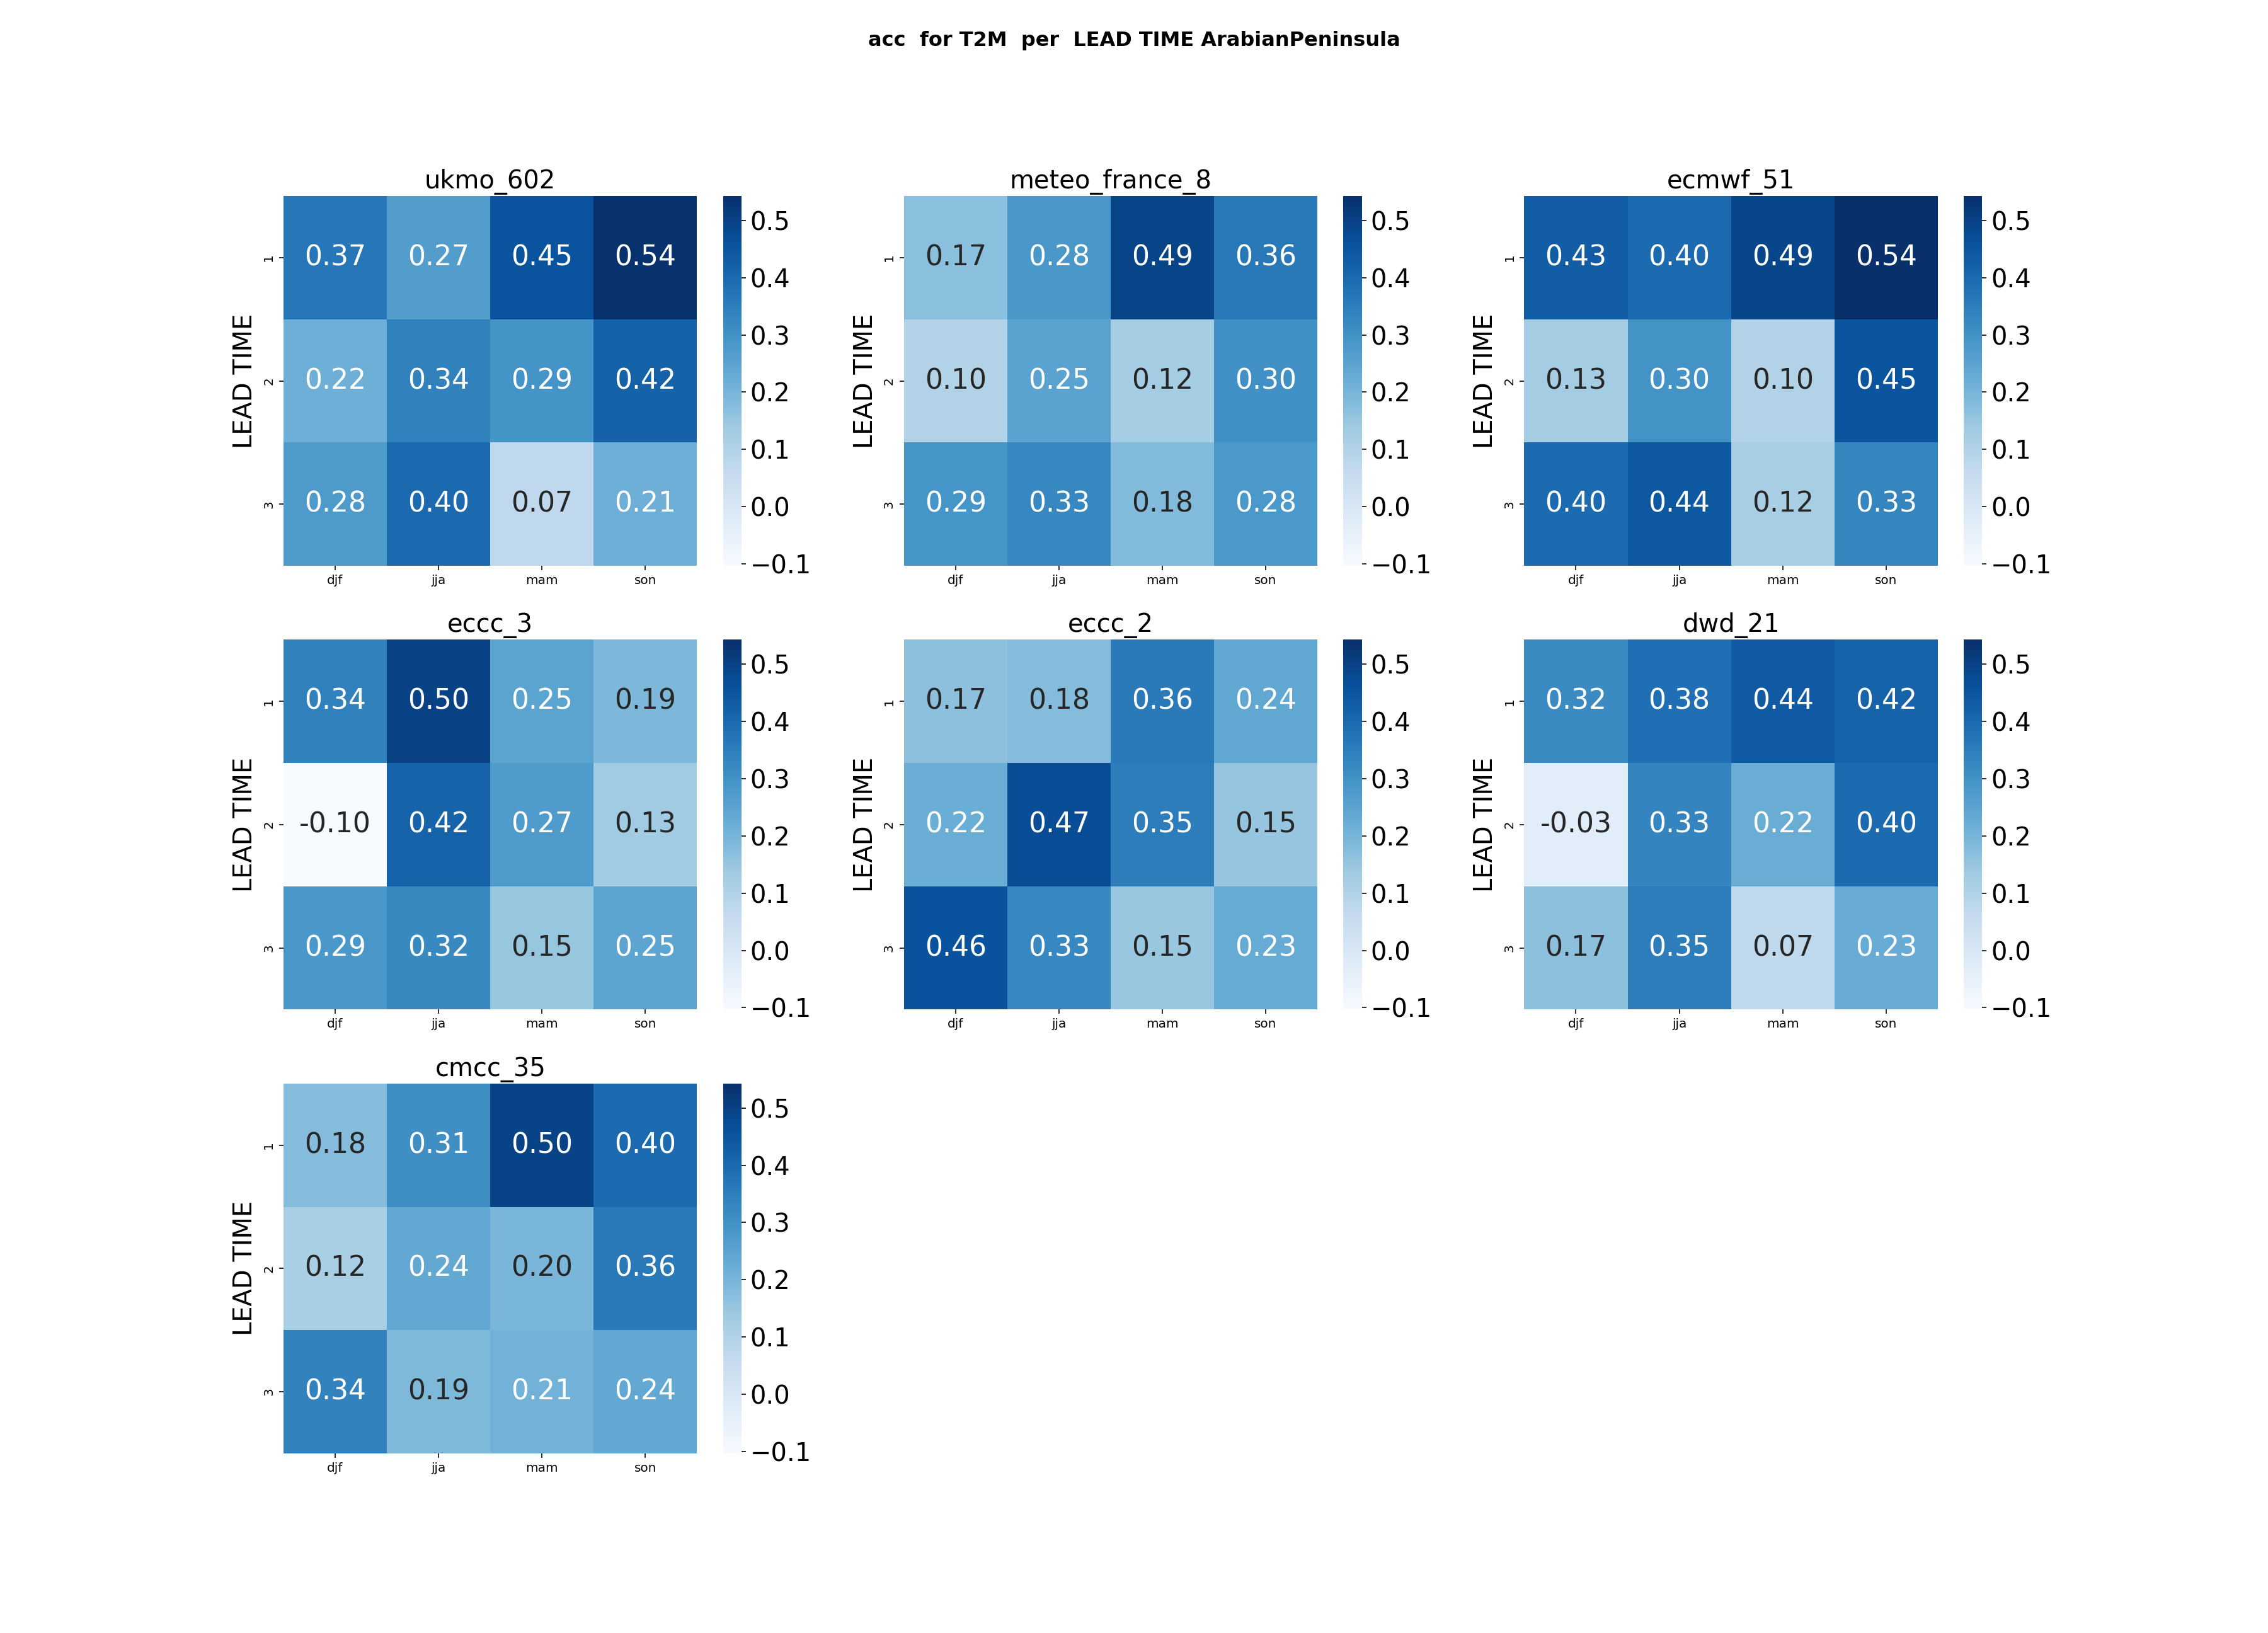
\includegraphics[scale=0.25]{plots/det/acc/acc_T2M_ArabianPeninsula.png}
\caption{ACC heatmap for the Arabian Peninsula across different periods \textbf{\textit{(1 indicates perfect correlation)}}.}
\end{figure}

The analysis highlights that the Arabian Peninsula consistently achieves better ACC scores compared to the general MENA region. Notably, the ACC is particularly high for \textbf{\textit{SON (September-October-November)}} at the third lead time.
\subsubsection{Analysis of RMSE Results}

\vspace{1.5cm}

\paragraph{focus on North Africa} : 
\begin{figure}[H]
\centering
\includegraphics[scale=0.3]{plots/det/rmse/rmse_T2M_NorthAfrica.png}
\caption{heatmap of RMSE For T2M  (North Africa)}
\end{figure}

The North African climate poses challenges for modeling extreme temperatures and spatial variability. Heatmap analysis shows that \textbf{\textit{ECMWF}} excels in JJA with RMSE values of 1.34°C–1.58°C but performs lower in other seasons. \textbf{\textit{Météo-France}} delivers consistent accuracy, especially in SON, making it more reliable for multi-seasonal forecasting in this region.
\vspace{1.5cm}
\paragraph{focus on Arabian Peninsula}:

\begin{figure}[H]
\centering
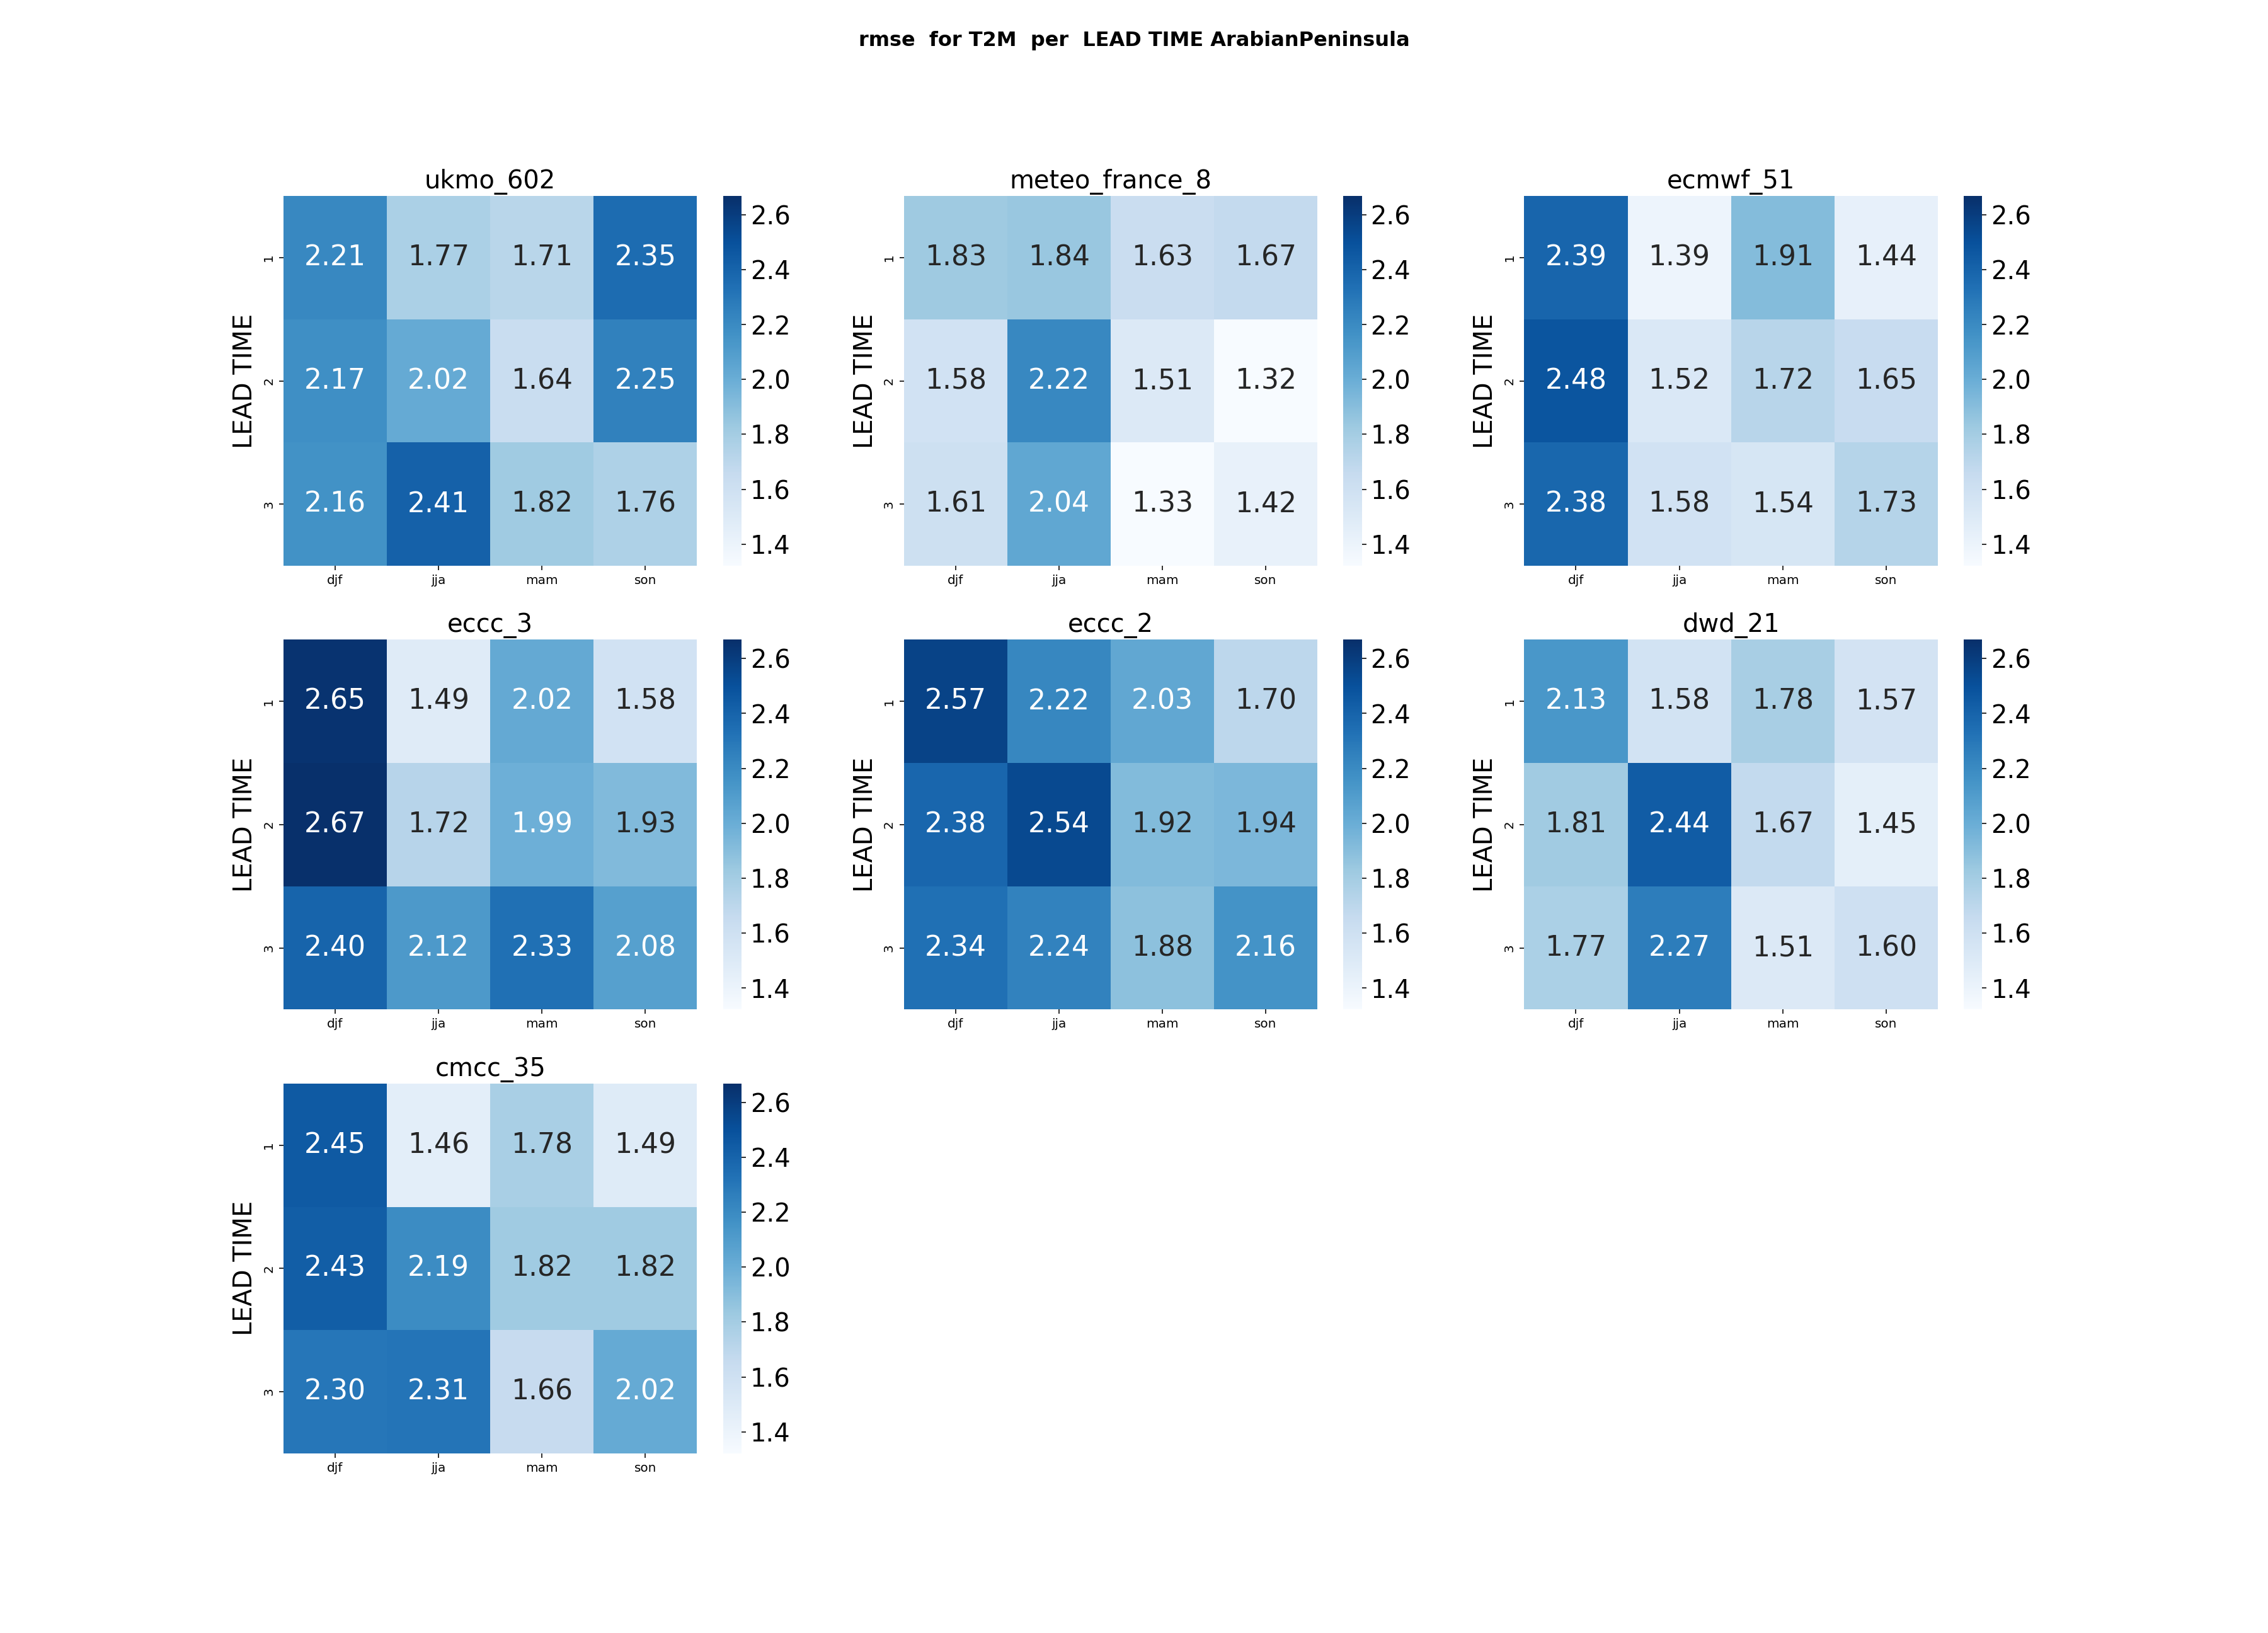
\includegraphics[scale=0.3]{plots/det/rmse/rmse_T2M_ArabianPeninsula.png}
\caption{heatmap of RMSE For T2M  (North Africa)}
\end{figure}

In the same way as North Africa, the RMSE for the Arabian Peninsula is significantly lower for \textbf{\textit{Météo-France}}, indicating superior performance.
\subsubsection{Analysis of Coefficient of Determination results}
\paragraph{focus on North Africa}

Focusing on North Africa, \textbf{\textit{ECMWF}} maintains its position as the most reliable center, consistent with its performance across the broader MENA region.
\begin{figure}[H]
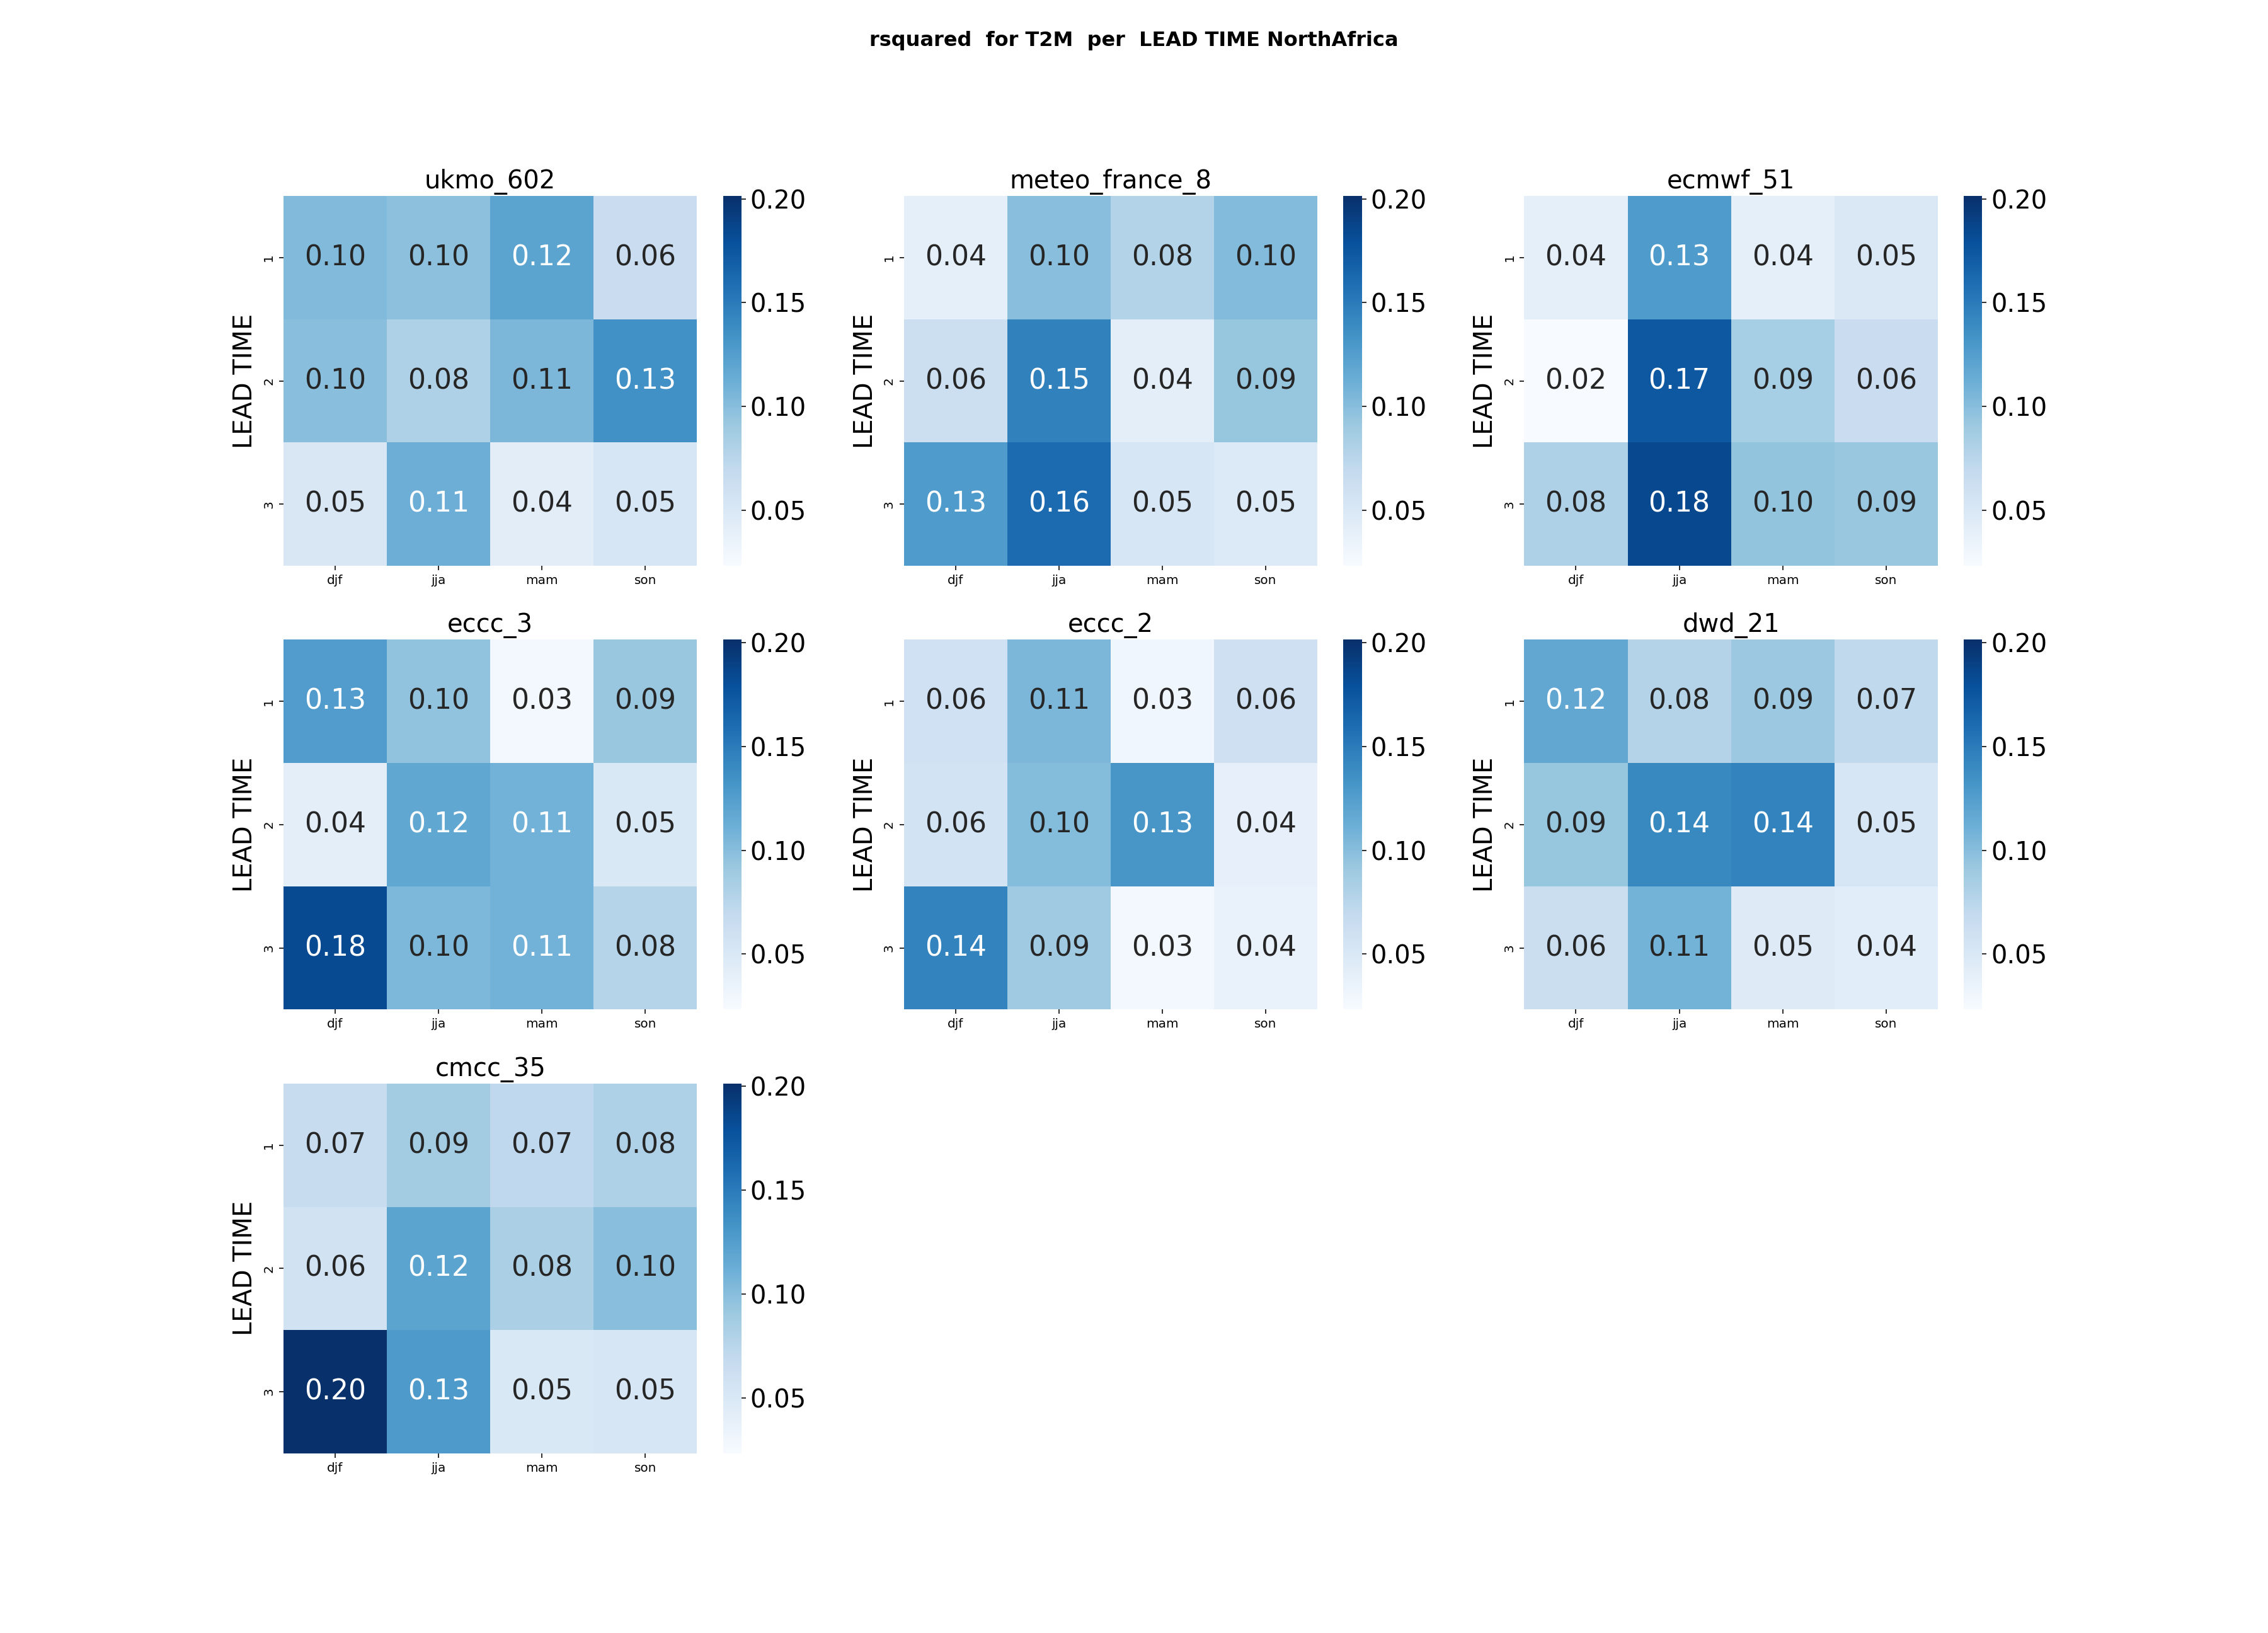
\includegraphics[scale=0.3]{plots/det/rsquared/rsquared_T2M_NorthAfrica.png}
\caption{Heatmap of T2M  RSQUARED in North Africa Region for all centers }
\end{figure}


\vspace{1.5cm}
\paragraph{focus on Arabian Peninsula}:


\begin{figure}[H]
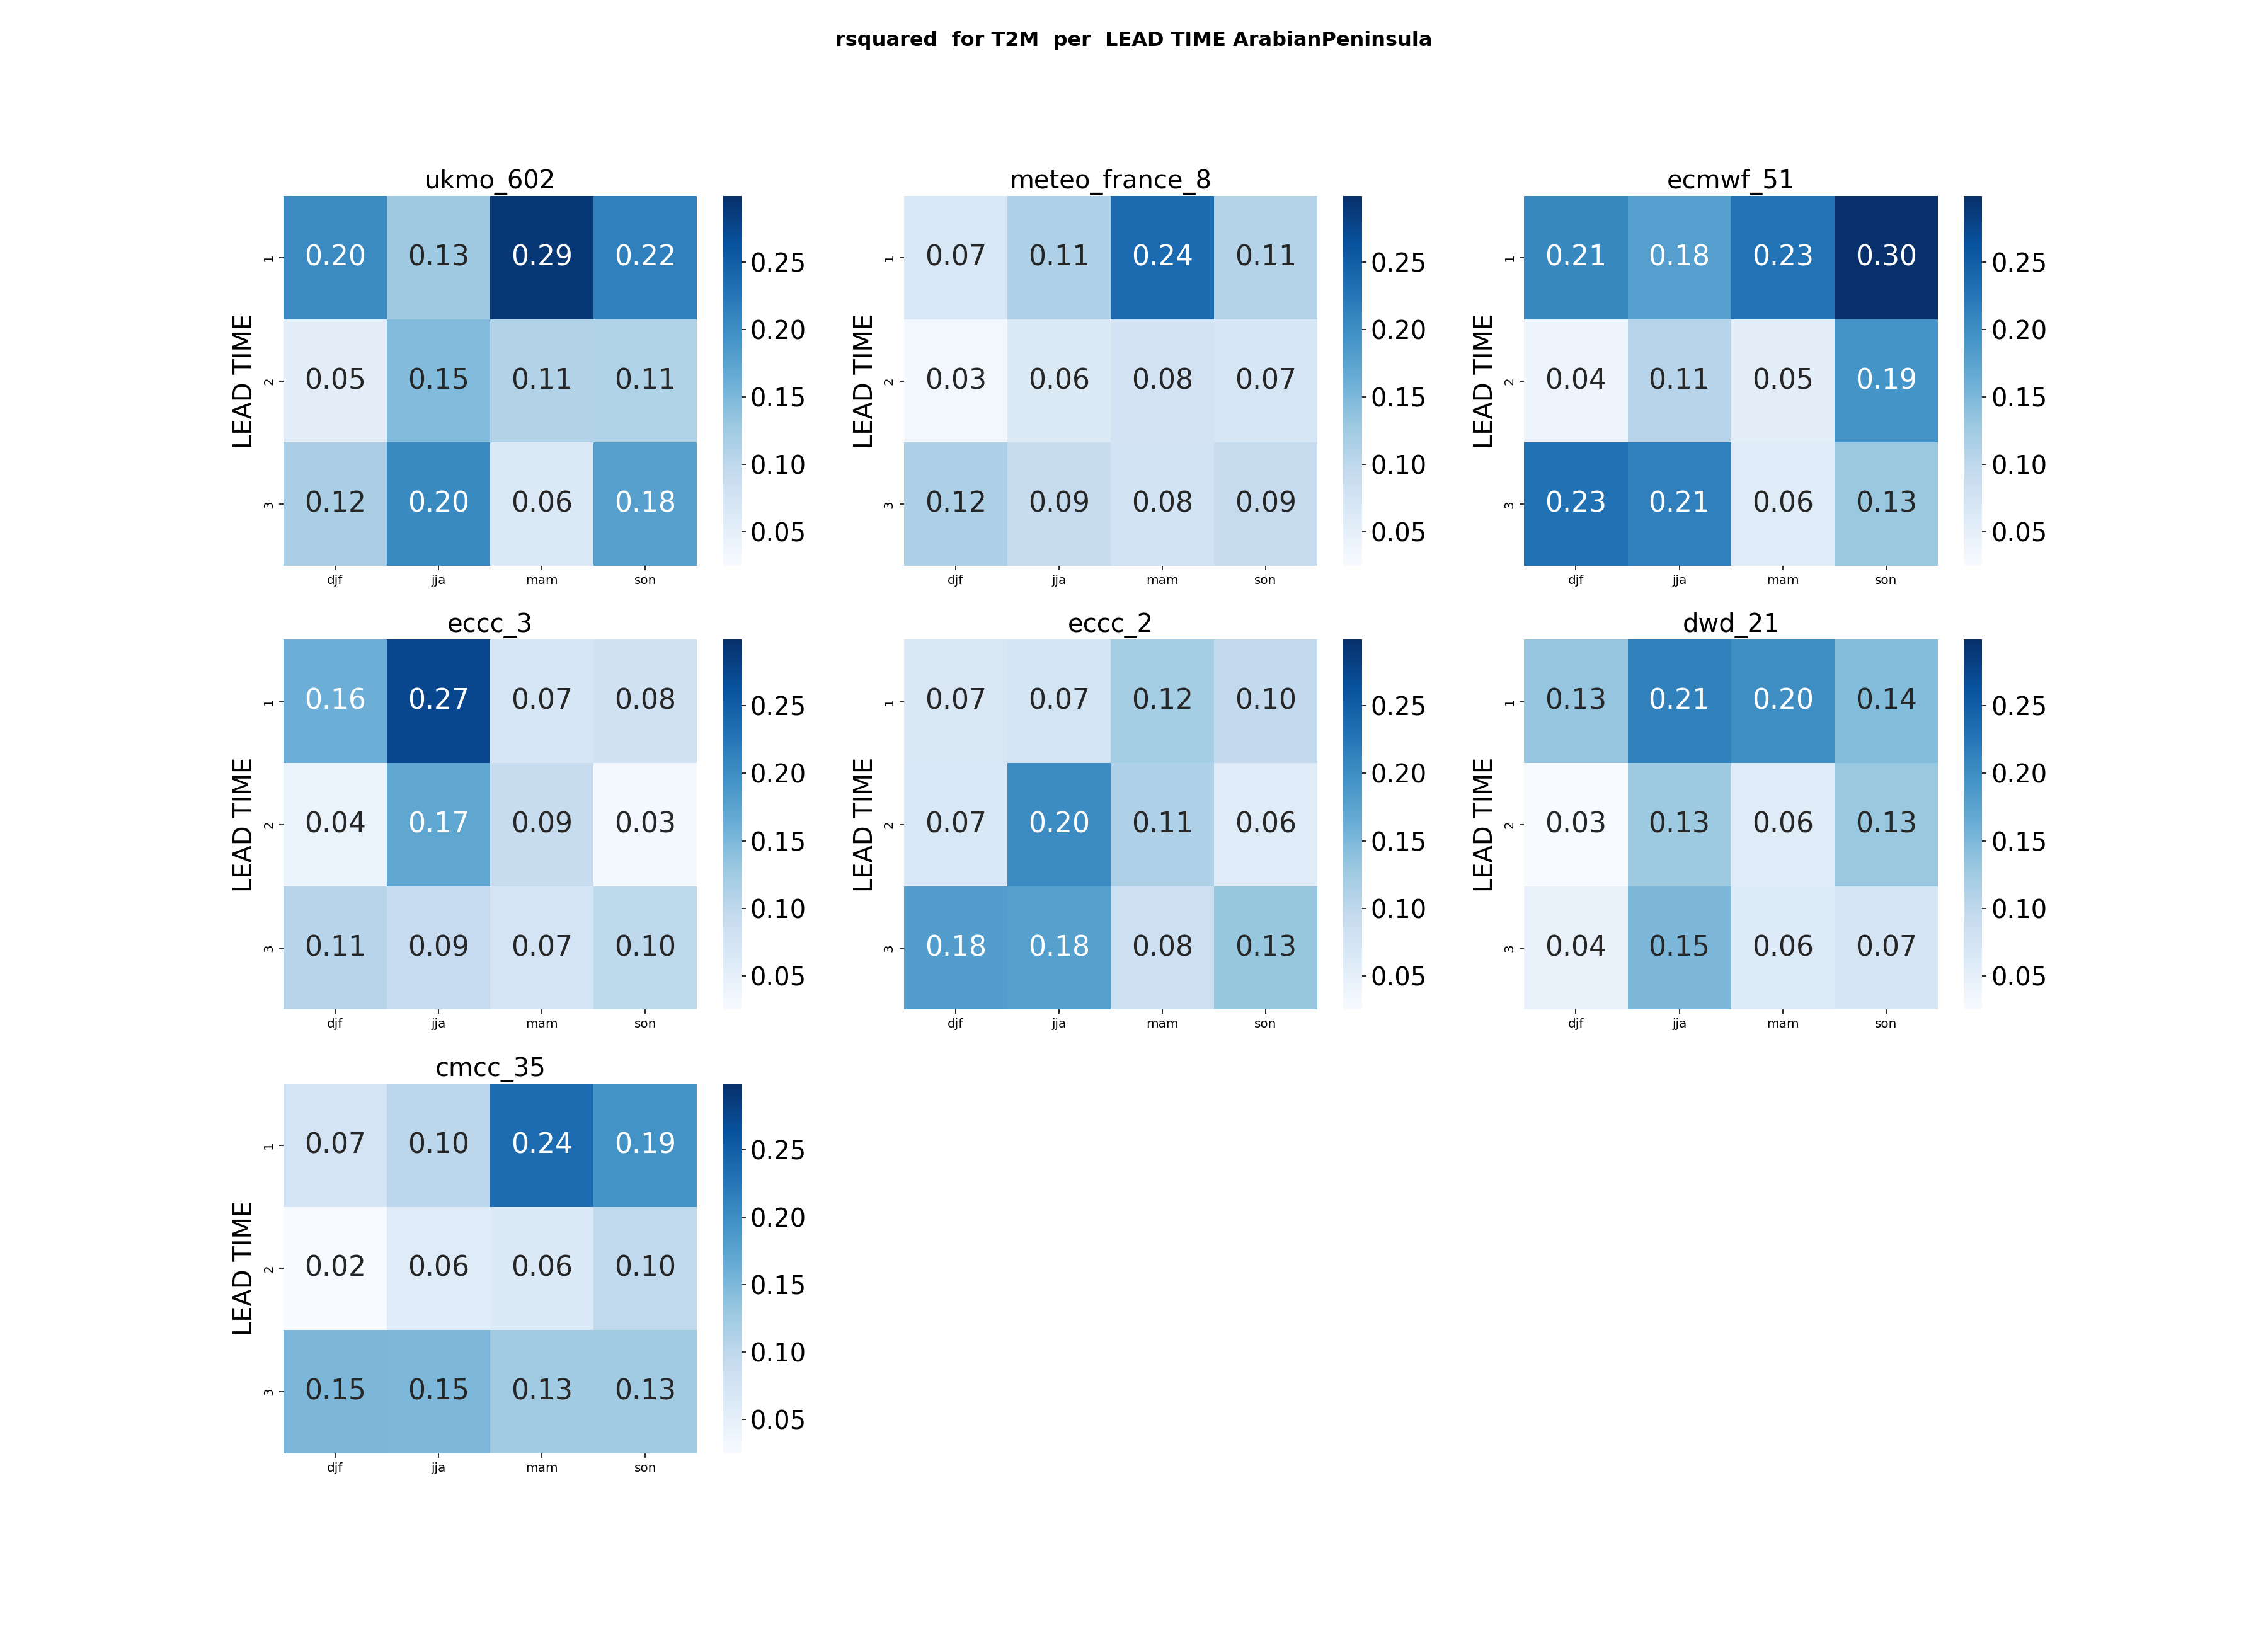
\includegraphics[scale=0.3]{plots/det/rsquared/rsquared_T2M_ArabianPeninsula.png}
\caption{Heatmap of T2M  RSQUARED in MENA Region for all centers Arabian Peninsula}
\end{figure}

the R-SQUARED for the Arabian Peninsula shows a little improvement.

\subsection{Probabilistic Evaluation Metrics}

\subsubsection{Analysis of The Brier Score results}

\paragraph{focus on North Africa}:

To evaluate model performance in North Africa, Brier Score analysis confirms that \textbf{\textit{ECMWF, CMCC, and Météo-France}} maintain low scores, reflecting consistent reliability across lead times and seasons. These findings indicate that North Africa’s unique climatic variability does not significantly impact the predictive skill of these models, affirming their adaptability within the broader MENA region. Minimal score variations across lead times further emphasize their robustness for accurate probabilistic forecasting over varying temporal ranges.

\begin{figure}[H]
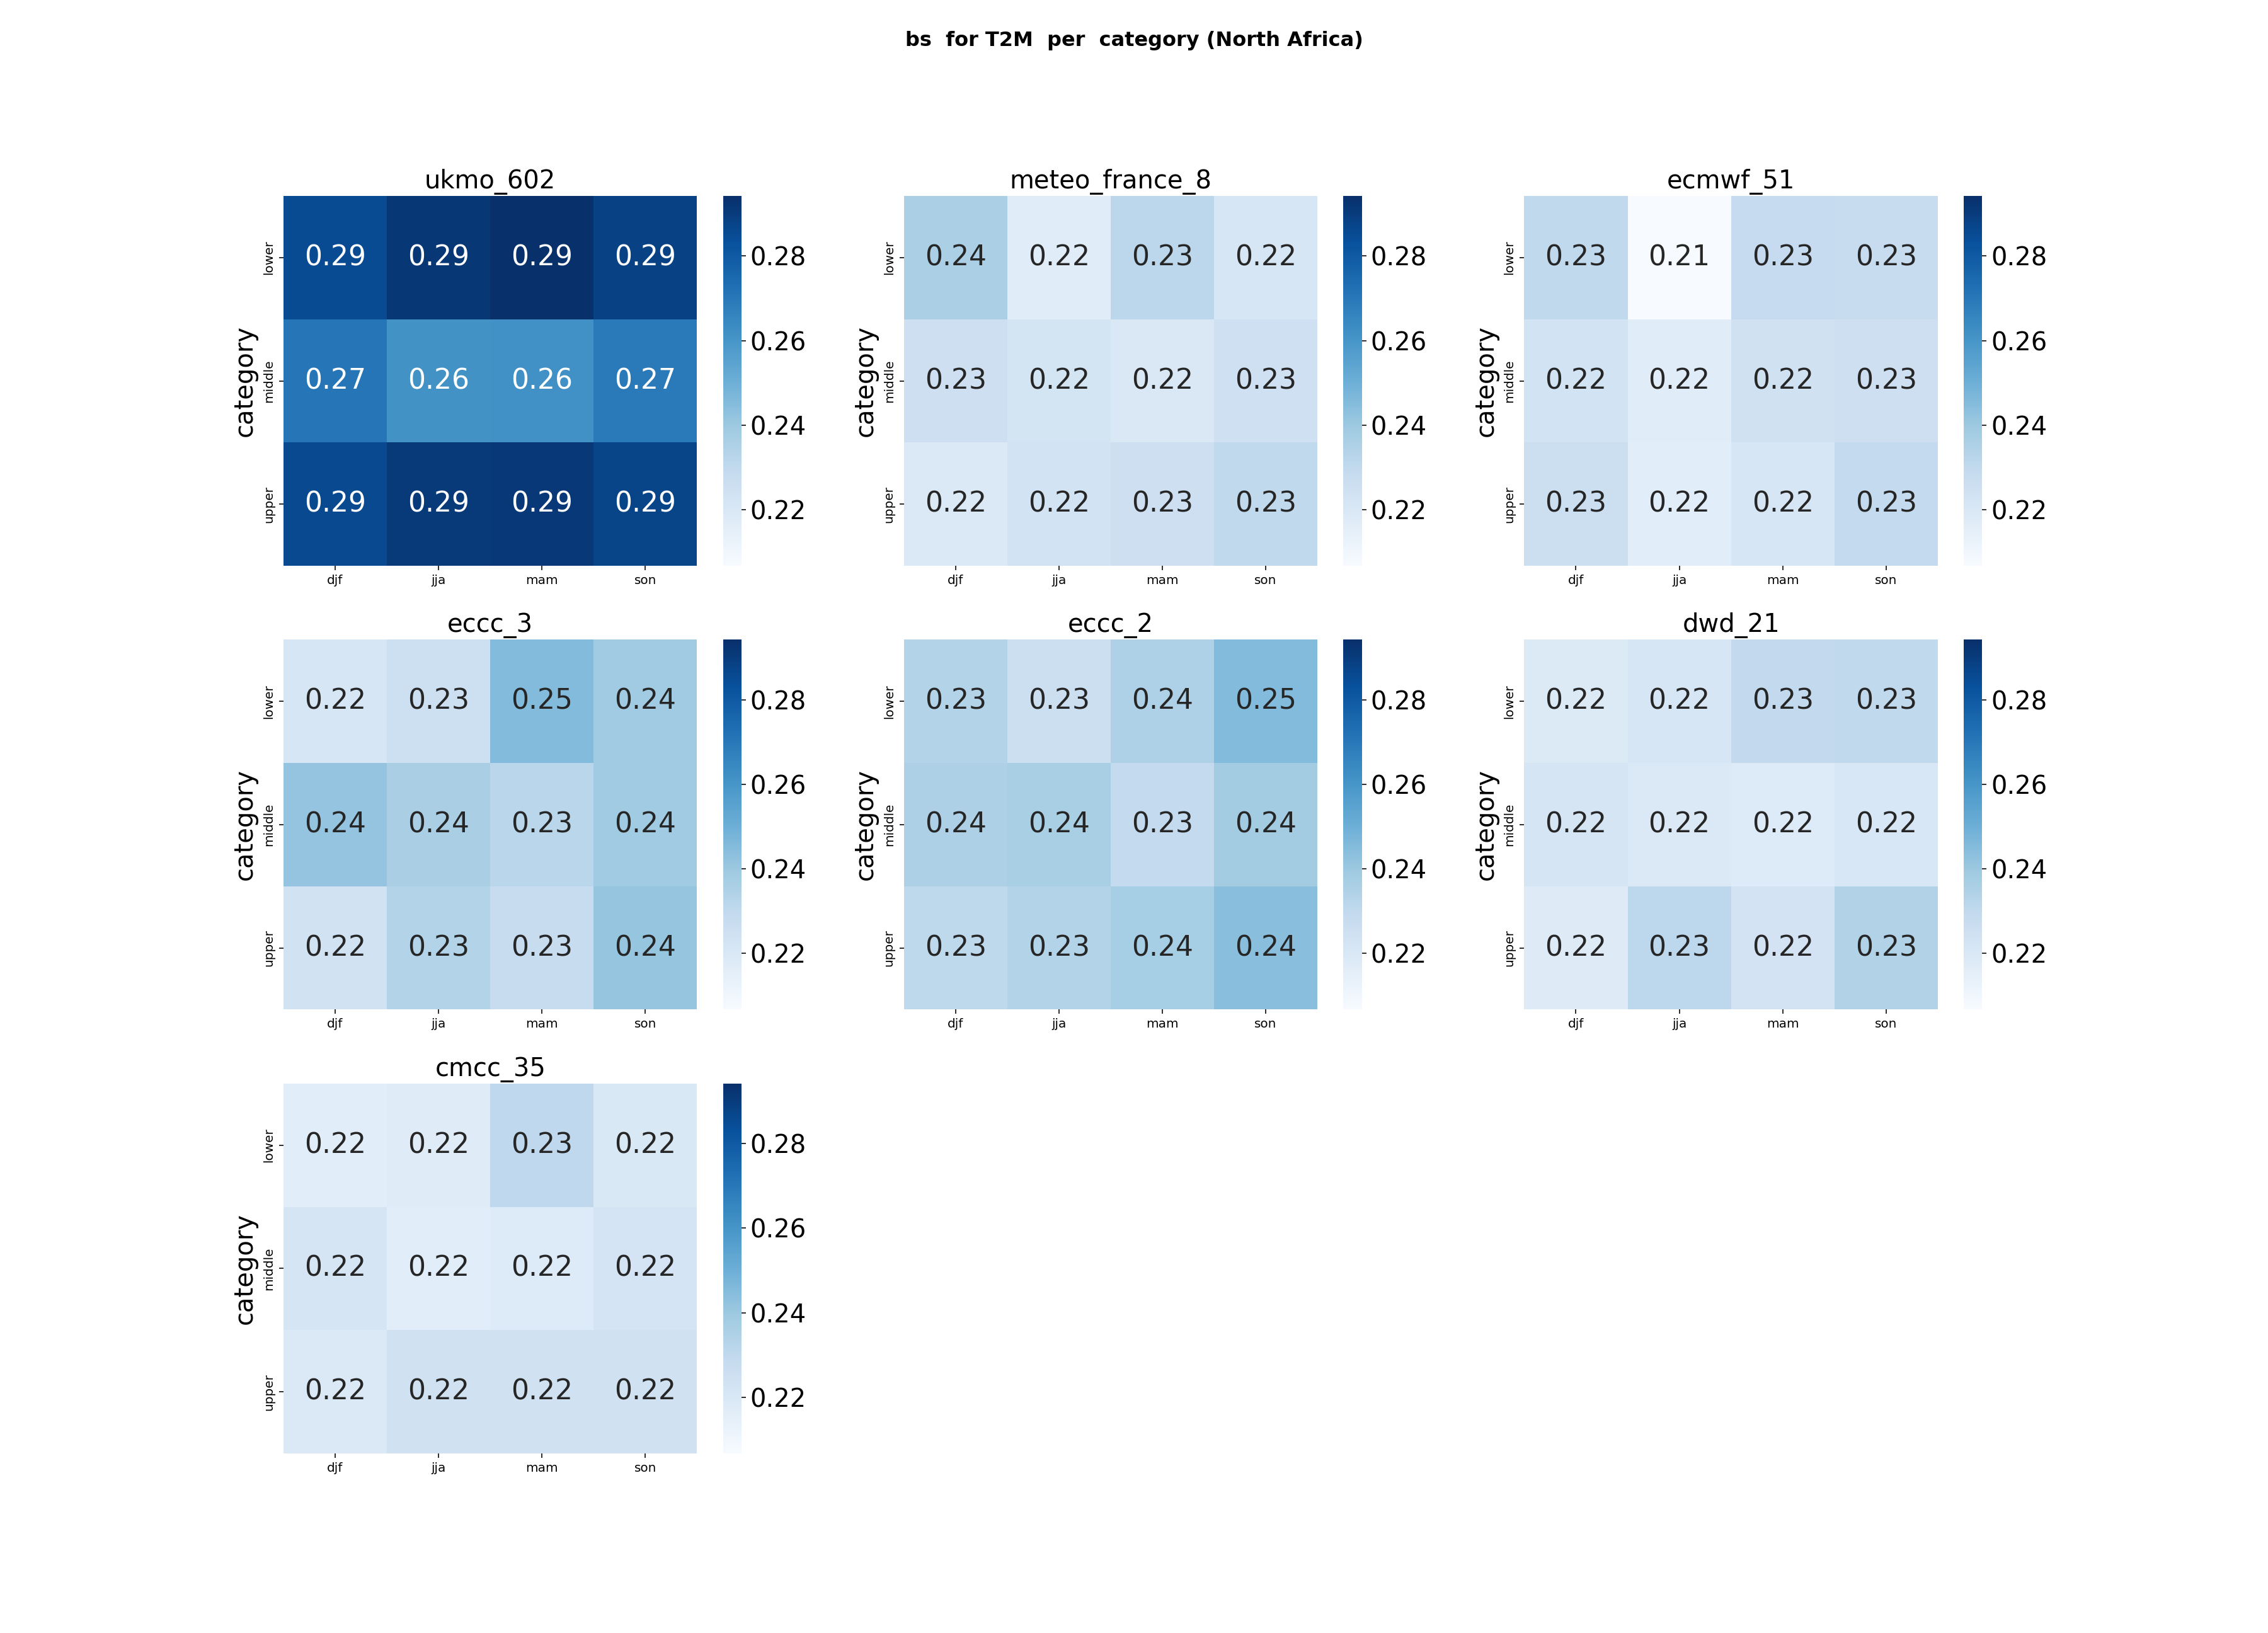
\includegraphics[scale=0.3]{plots/prob/bs/bs_T2M_category_NorthAfrica.png}

\caption{Heatmap of T2M  brier score for all centers in North Africa region}
\end{figure}





\vspace{1.5cm}
\paragraph{focus on Arabian Peninsula}:
there is no big difference in North Africa.
\subsubsection{Analysis of Reliability results}
\paragraph{focus on North Africa}:
\begin{figure}[H]
\includegraphics[scale=0.3]{plots/prob/rela/rela_T2M_NorthAfrica.png}

\caption{Heatmap of T2M  reliability  for all centers in North Africa}
\end{figure}


A more focused analysis on North Africa has not significantly altered the overall conclusions derived from the broader MENA region. The consistent performance patterns observed across the different models and seasons remain largely unchanged when examining the North African context. 

\paragraph{focus on Arabian Peninsula}:

there is no big difference in  Arabian Peninsula.
\subsubsection{Analysis of The ranked probability score results}
\paragraph{focus on north africa:}
For the North African region, the results mirror those observed in the broader MENA region.  

This suggests that despite the localized focus on North Africa, the model performance differences remain significant, particularly for UKMO. 

\begin{figure}[H]
\includegraphics[scale=0.3]{plots/prob/rps/rps_T2M_NorthAfrica.png}

\caption{Heatmap of T2M  rps  for all centers in North Africa regions}
\end{figure}


\paragraph{focus on Arabian Peninsula}:
All centers exhibit nearly identical performance, with the exception of \textit{UKMO}, which demonstrates lower skill compared to the others.
\subsubsection{Analysis of Receiver Operating Characteristic results}
\paragraph{focus on north africa:}
\begin{figure}[H]
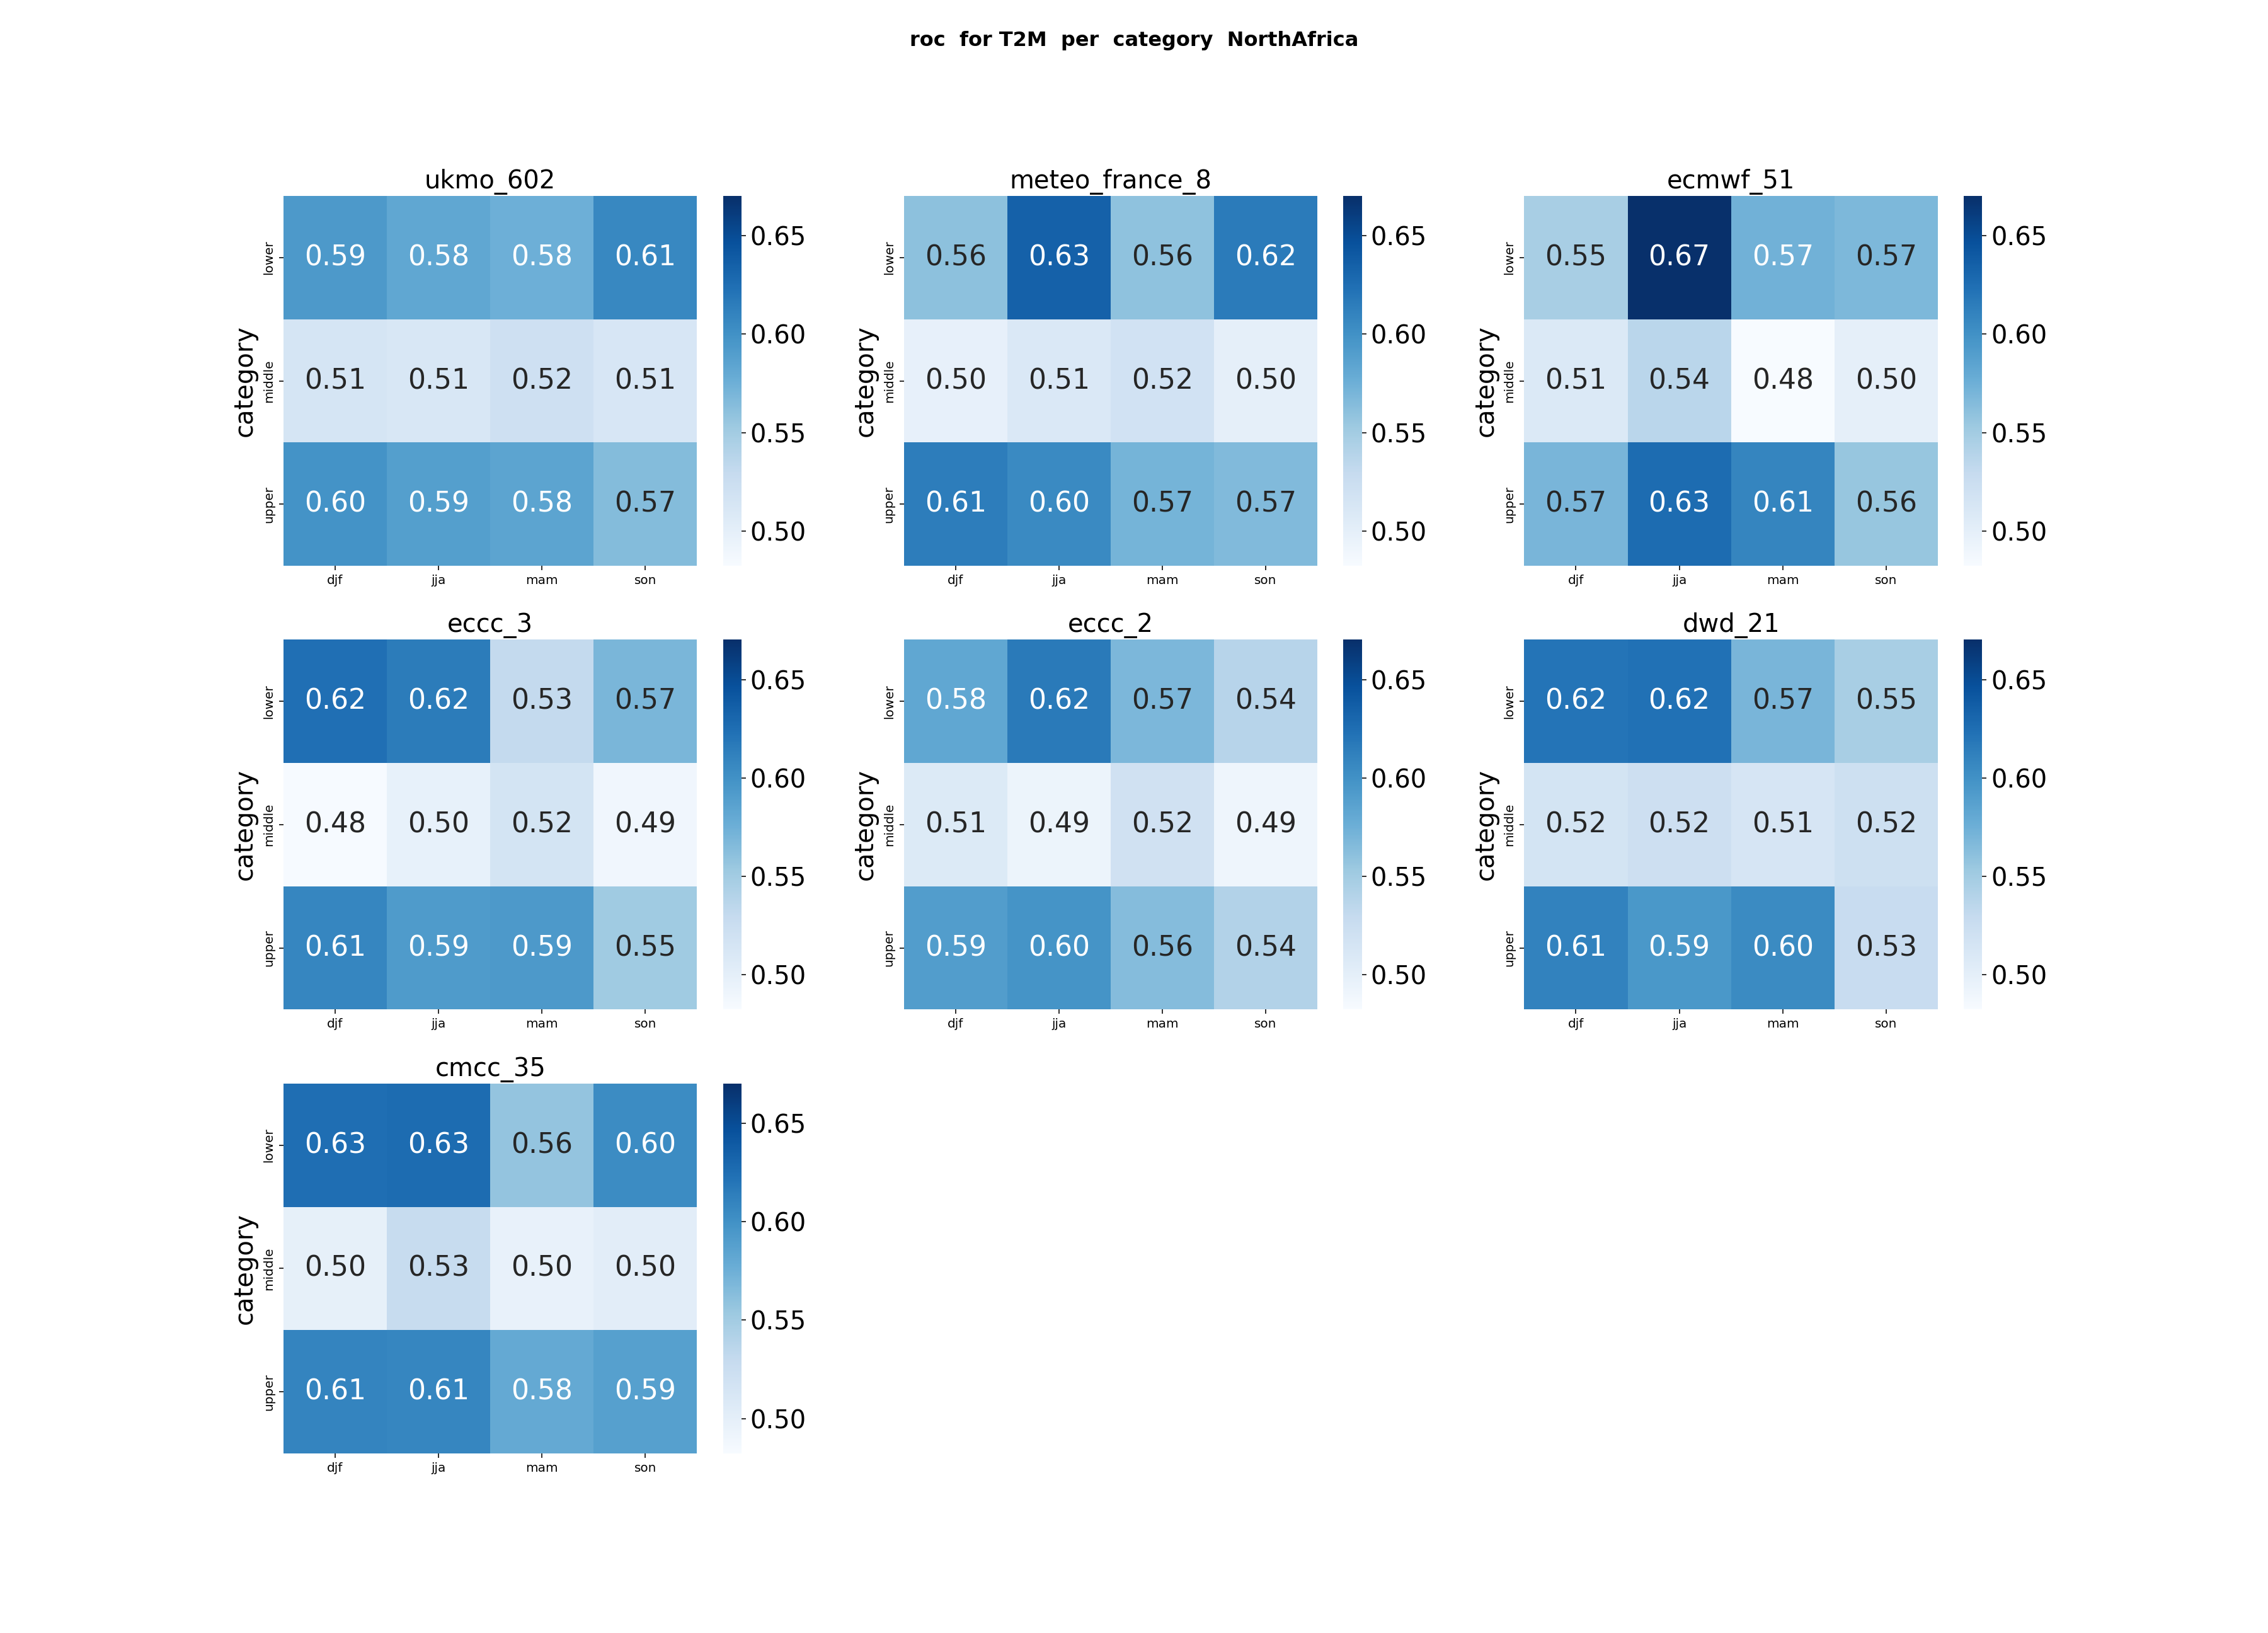
\includegraphics[scale=0.3]{plots/prob/roc/roc_T2M_category_NorthAfrica.png}

\caption{Temperature AUC  heatmaps for north africa }
\end{figure}

The figure above confirms the same conclusions for the North Africa region. The models generally maintain similar performance, with high AUC values reflecting strong discrimination skill across all categories. UKMO continues to show robust results in terms of ROC, despite its weaker reliability performance. As observed previously, the "middle" probability category remains the least performant compared to the "lower" and "upper" categories, indicating the models' reduced ability to predict moderate probability events. This consistency in findings suggests that the regional focus on North Africa does not significantly alter the overall assessment of model performance.
\paragraph{focus on Arabian Peninsula}:
There are no significant differences in performance across the centers, indicating comparable skill levels.
\subsubsection{Analysis of Relative operating characteristics Skill Score results }
\paragraph{focus on north africa:}
The ROC Skill Score (ROCSS) analysis reveals similar conclusions to the ROC results for Mena region and north Africa. 
\begin{figure}[H]
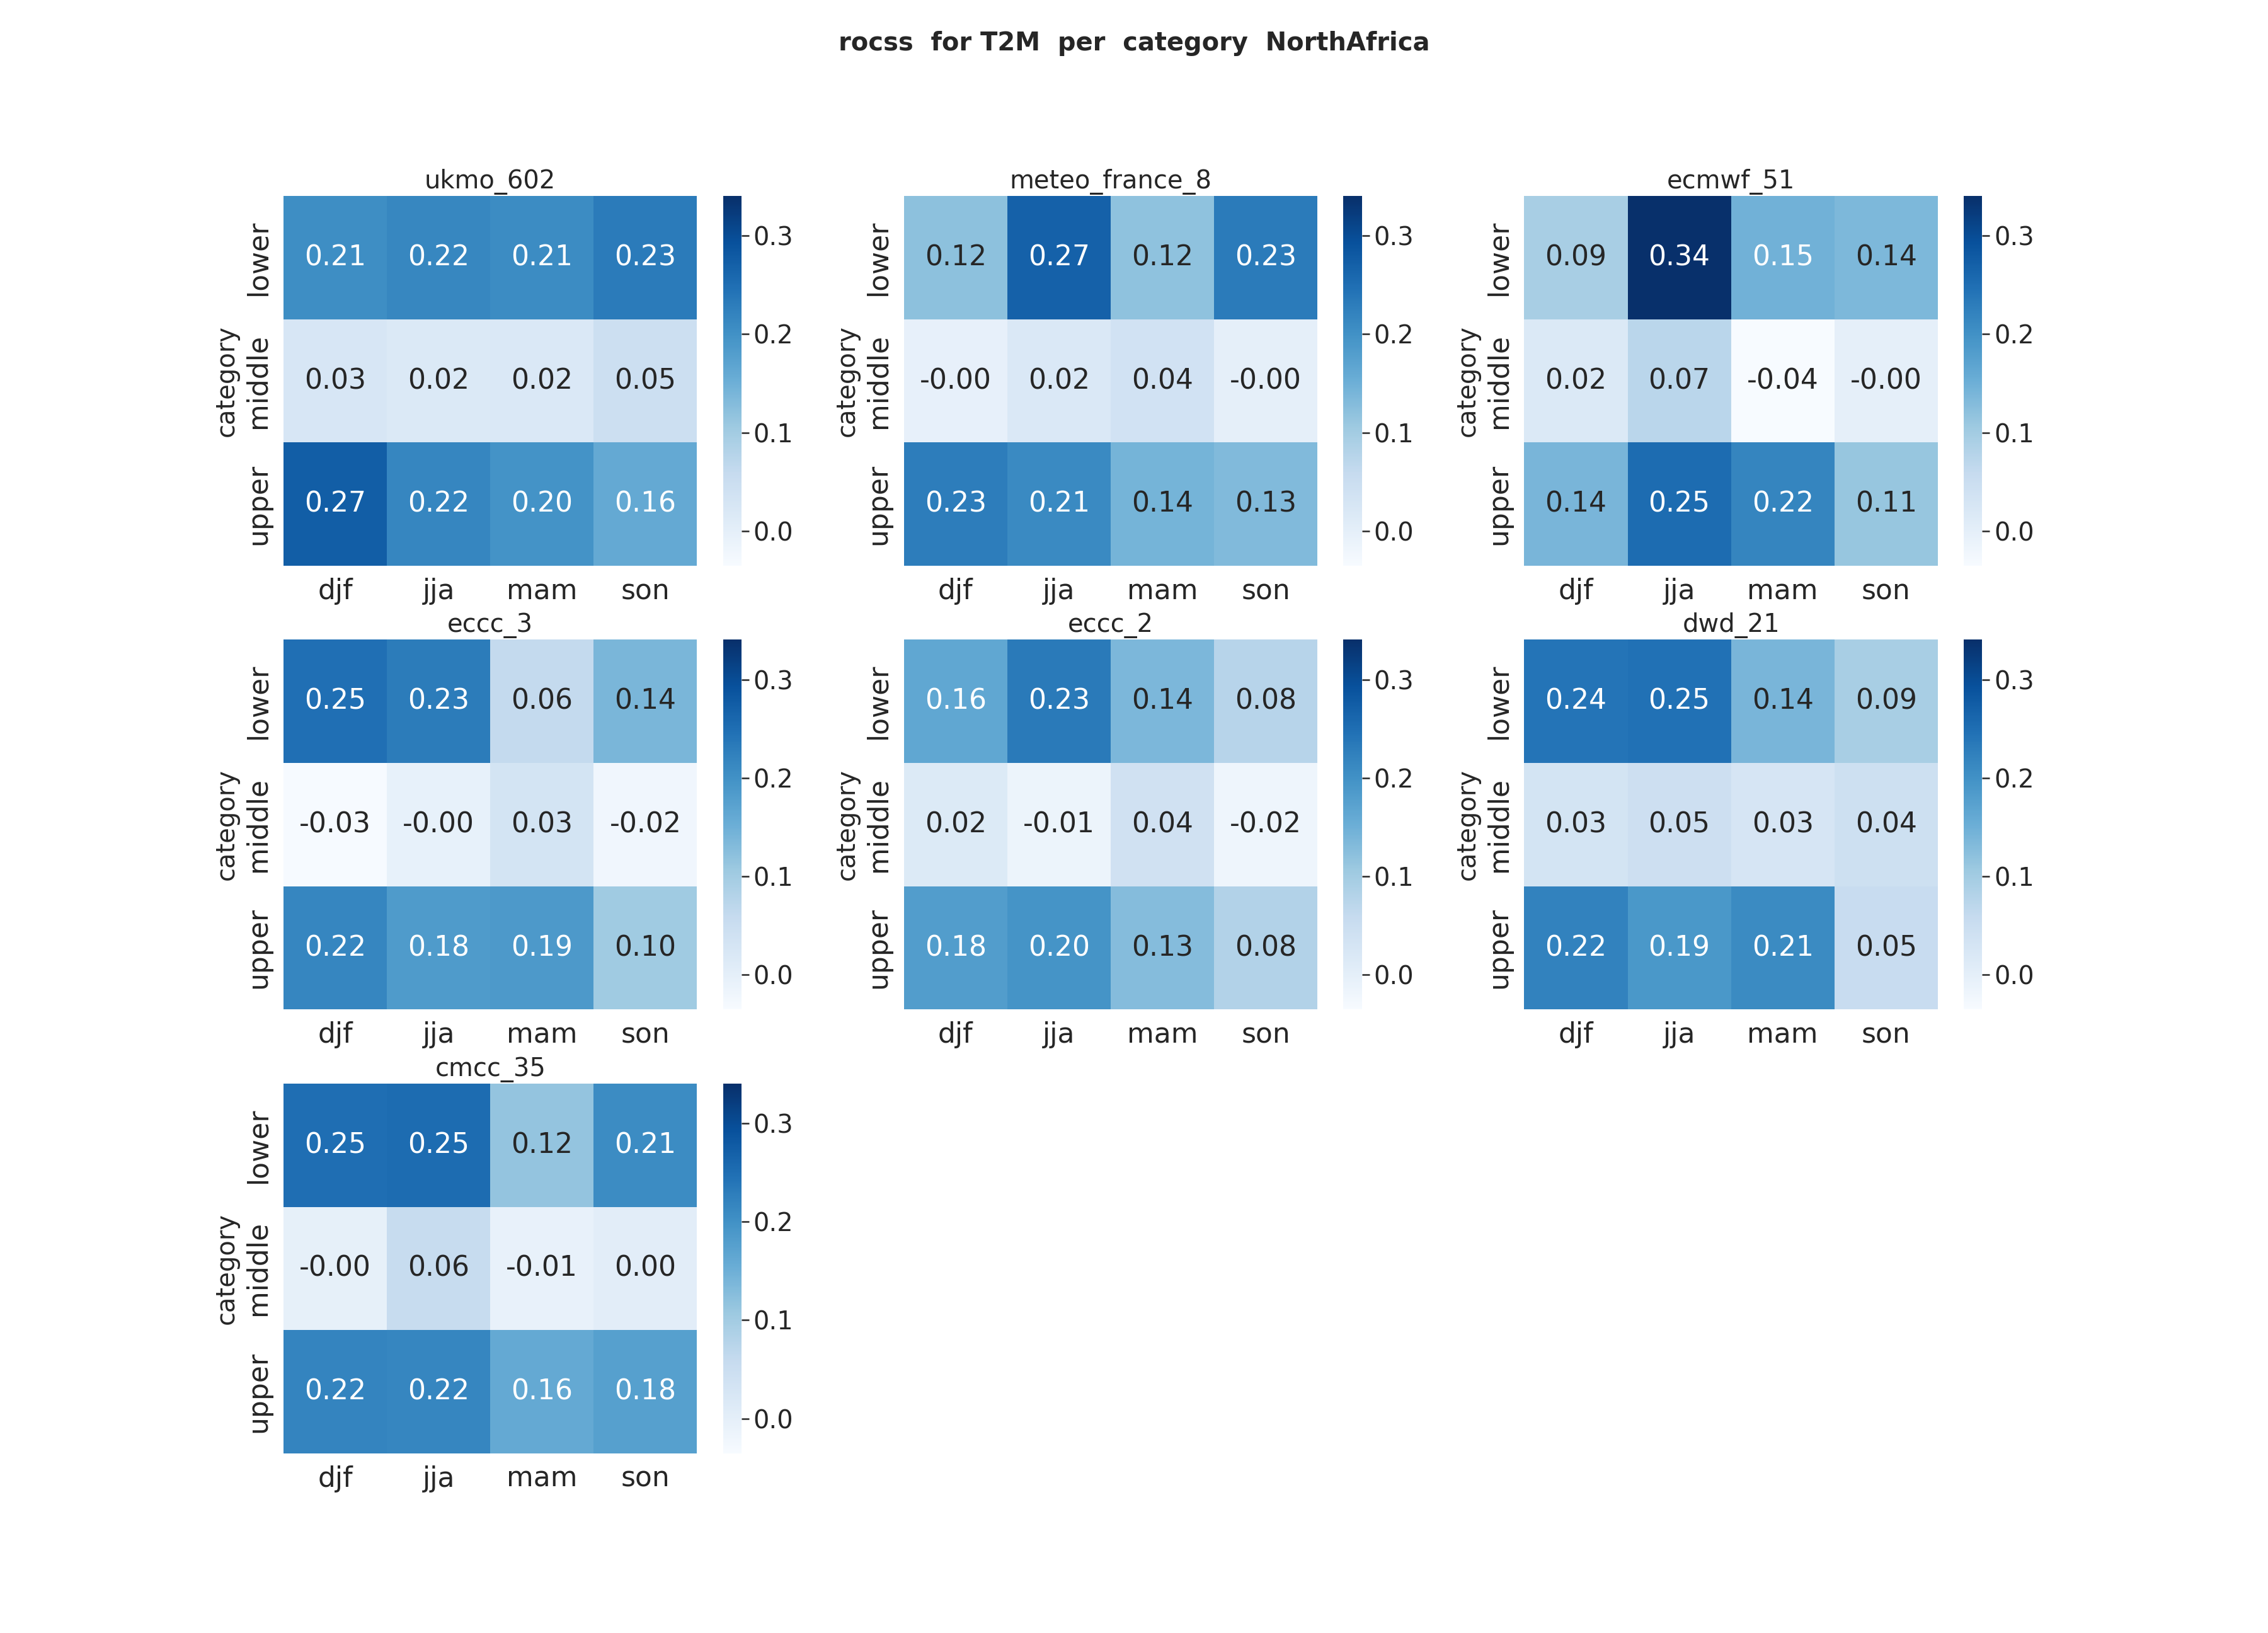
\includegraphics[scale=0.3]{plots/prob/rocss/rocss_T2M_category_NorthAfrica.png}

\caption{Temperature ROCSS  heatmaps for north africa }
\end{figure}

\paragraph{focus on Arabian Peninsula}:
There are no significant differences



\section{precipitation}
\subsection{Deterministic Evaluation Metrics}
\subsubsection{Analysis of ACC results}
 

\paragraph{focus on north africa:}
according to the heatmap below, the correlation shows no big difference for the first lead-time, but for the second and third lead-times, it became lower. Thus, the \textbf{\textit{ecmwf,ukmo and meteo-france}} maintain relatively good correlation.


\begin{figure}[H]
	\centering
	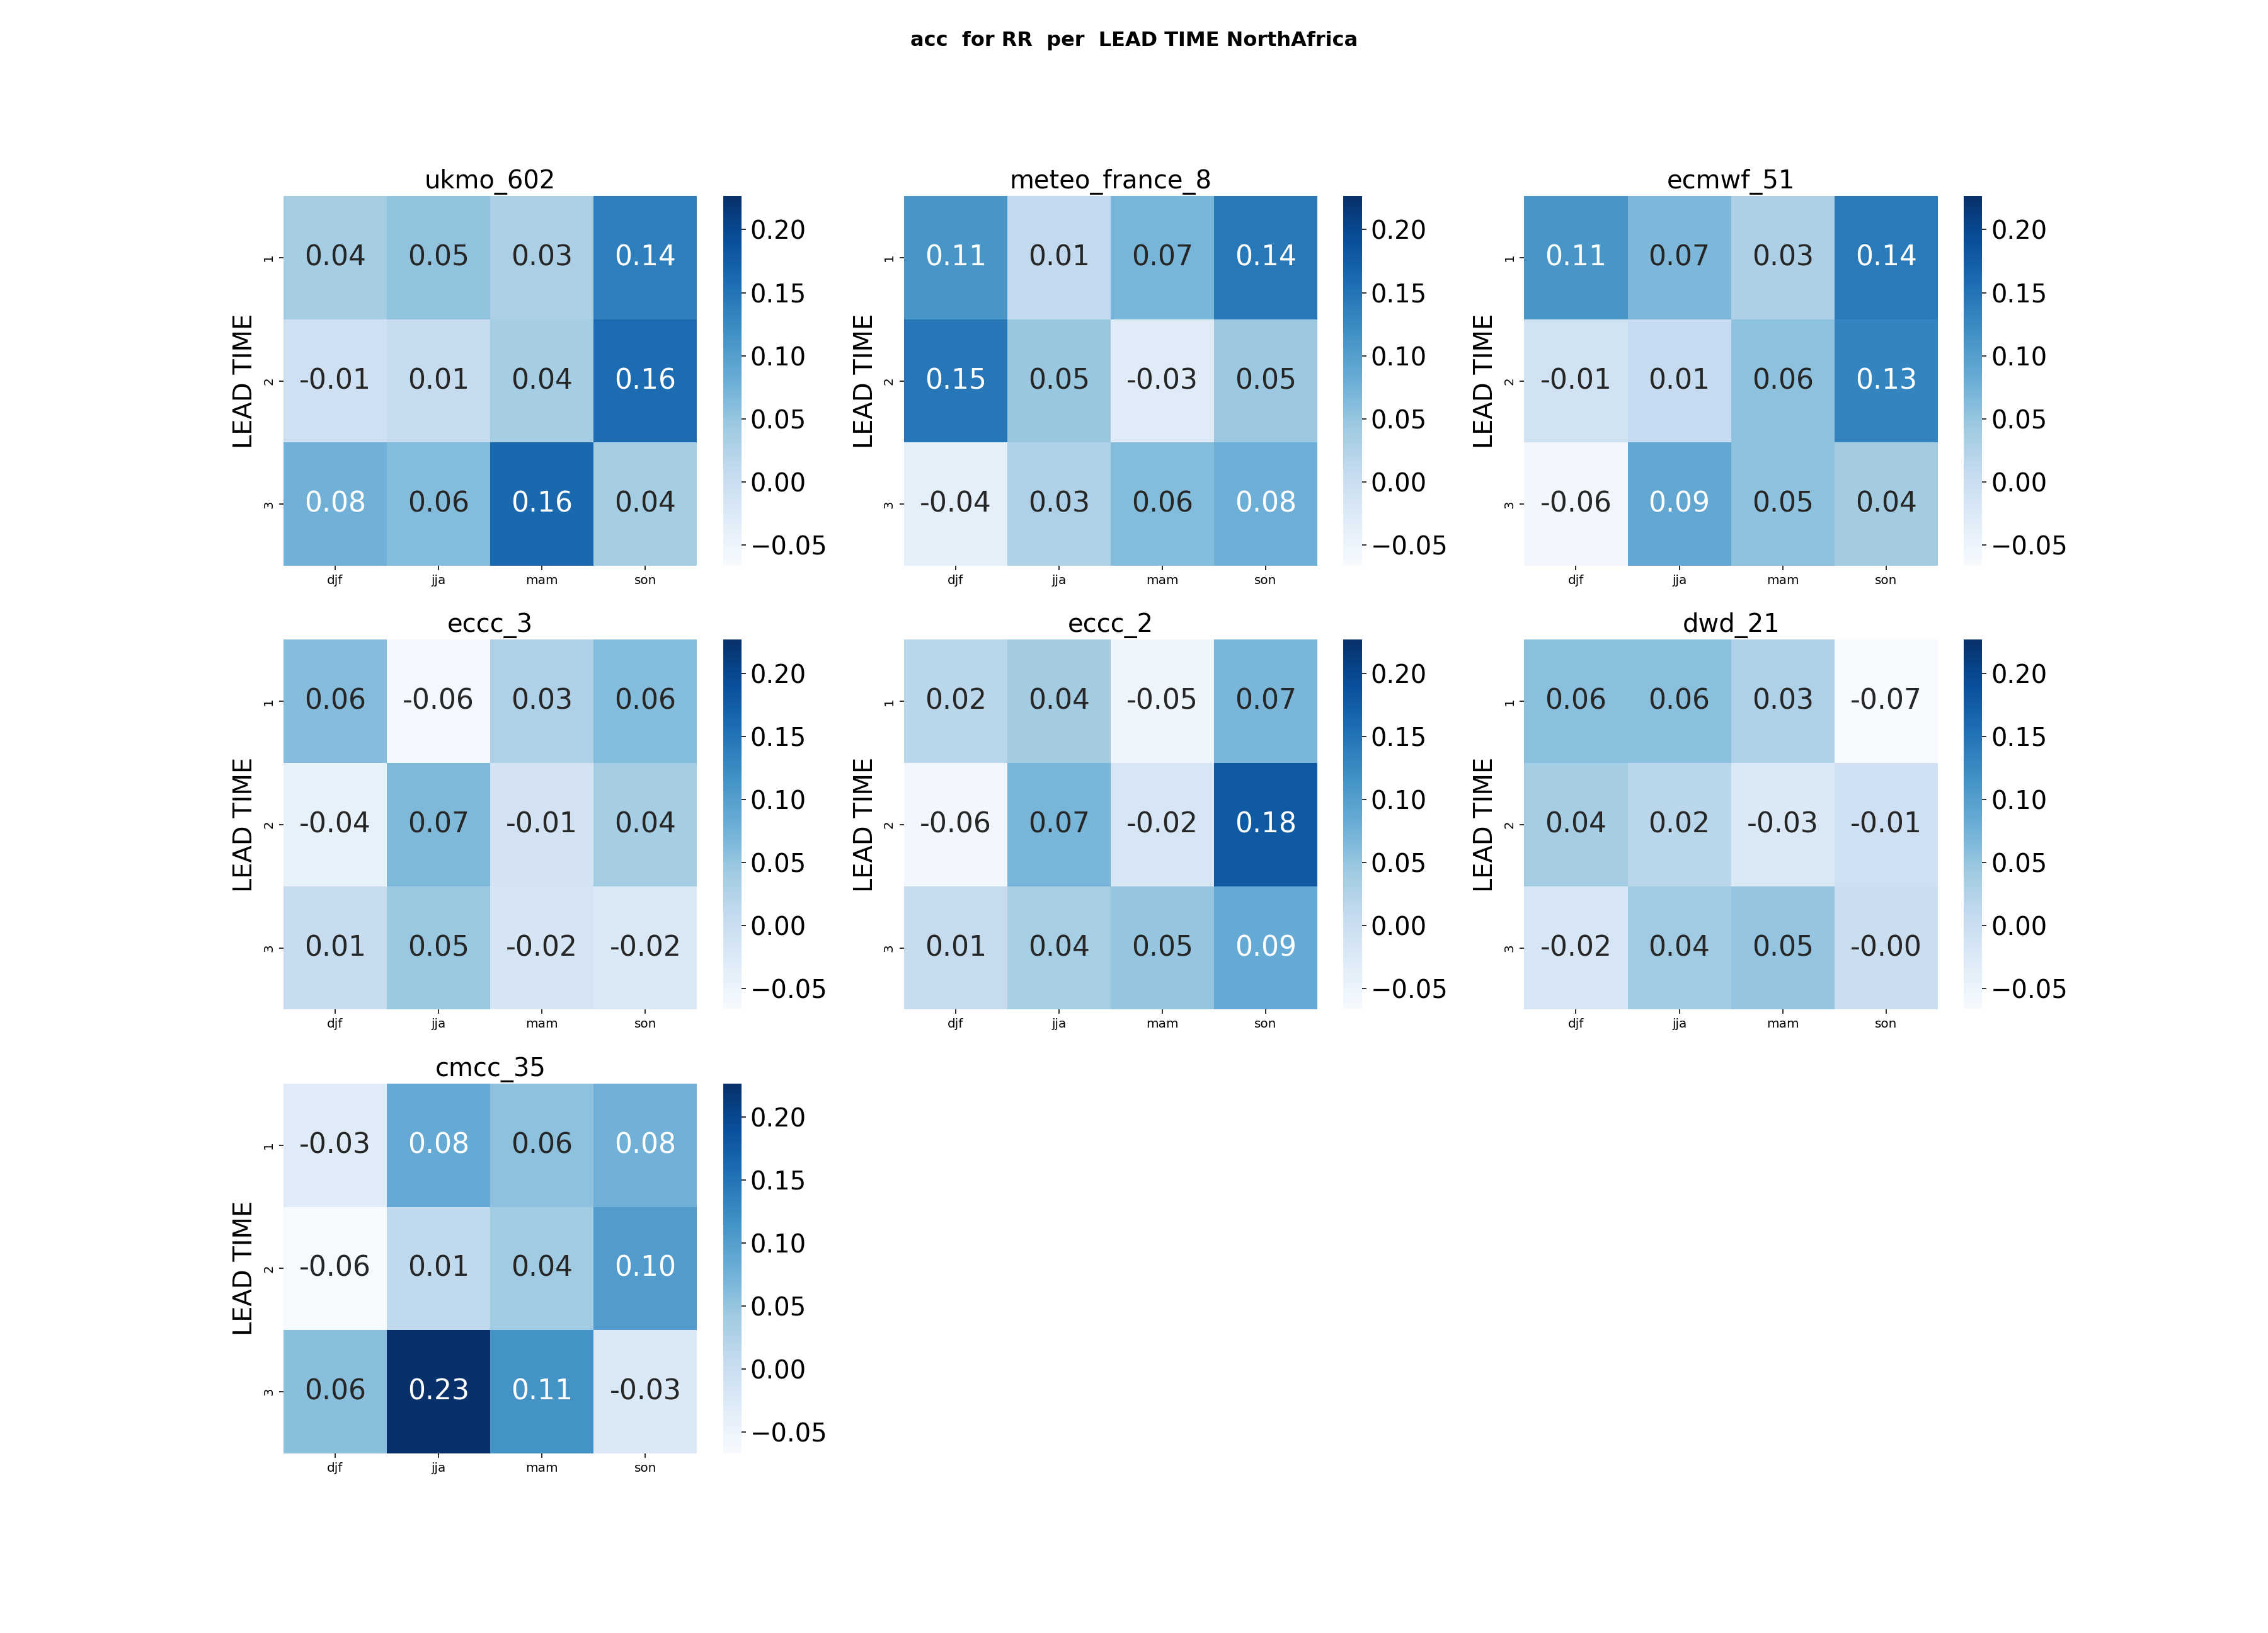
\includegraphics[scale=0.25]{plots/det/acc/acc_RR_NorthAfrica.png}
	\caption{The Heatmap of ACC for the North Africa region for every period \textbf{\textit{(1 for perfect Correlation)} }}
\end{figure}

\vspace{1.5cm}
\paragraph{focus on Arabian Peninsula}:

\begin{figure}[H]
	\centering
	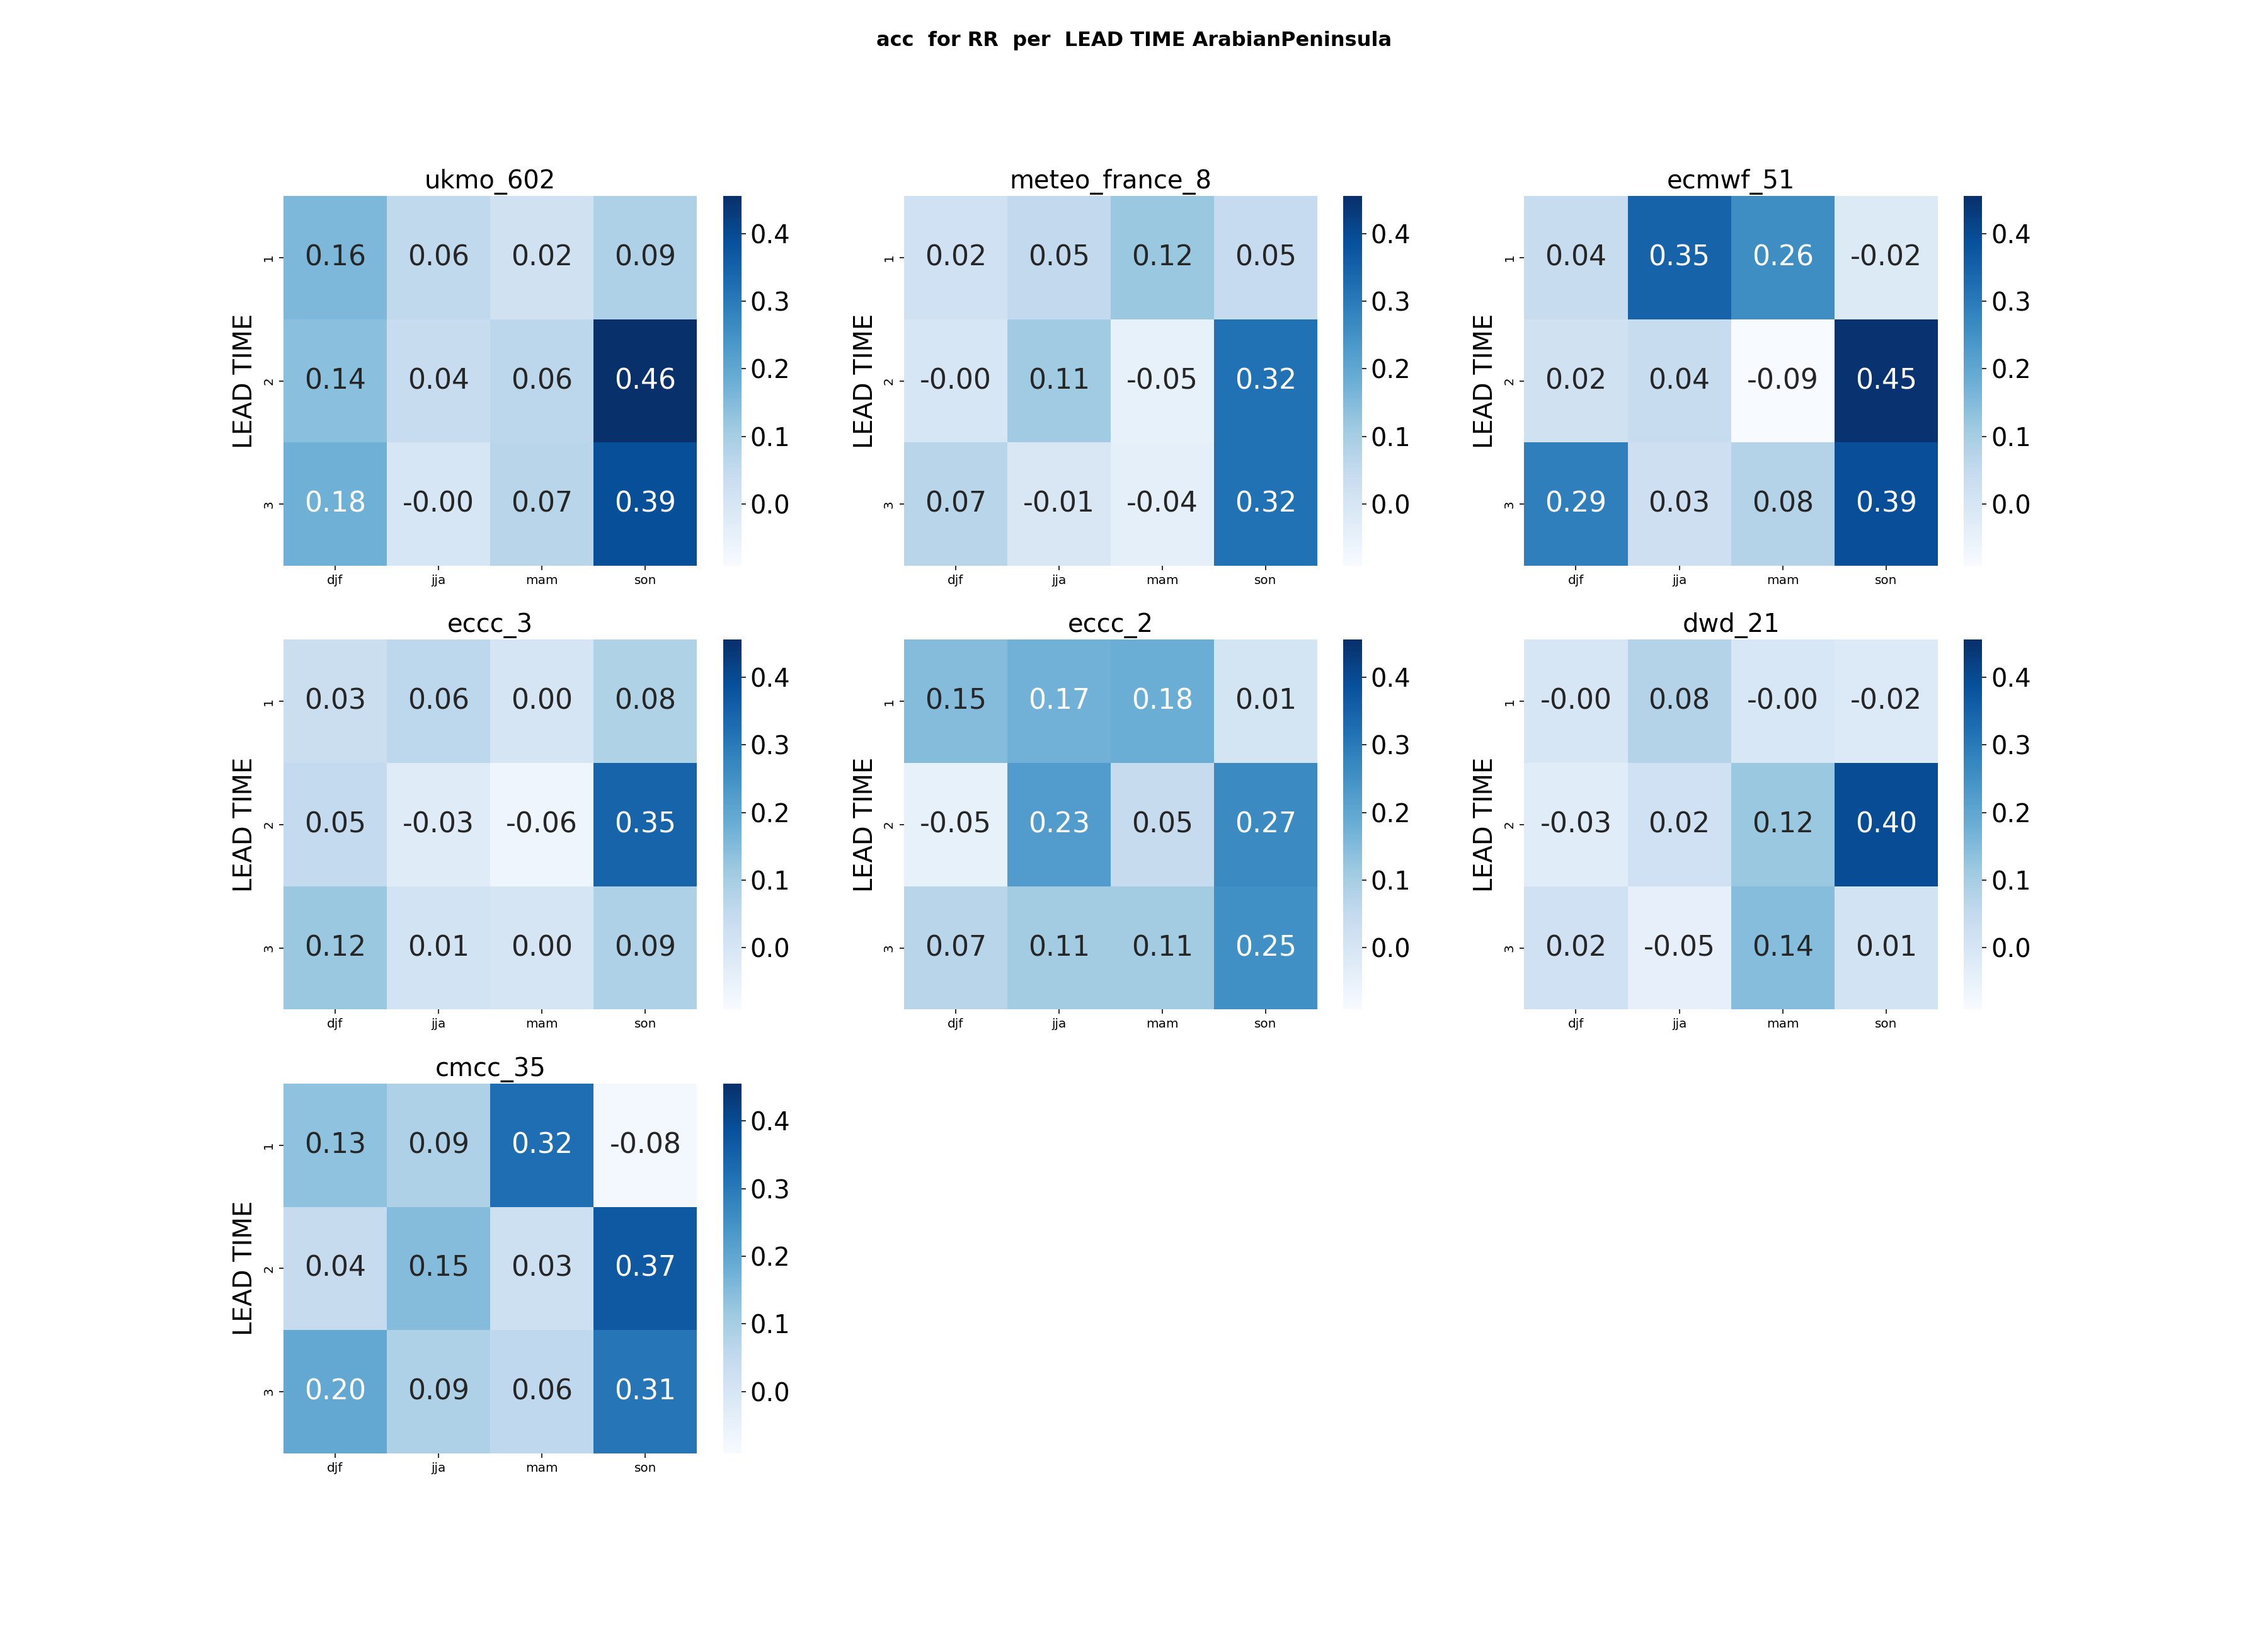
\includegraphics[scale=0.25]{plots/det/acc/acc_RR_ArabianPeninsula.png}
	\caption{The Heatmap of acc for the Arabian Peninsula region for every period  \textbf{\textit{(1 for perfect ACC)} }}
\end{figure}

The analysis of the Arabian Peninsula shows that the score is much better than the general situation of the mena region. The acc is good especially for SON for the second and third lead-times.
\subsubsection{Analysis of RMSE Results}

\vspace{1.5cm}

\paragraph{focus on North Africa} : 
\begin{figure}[H]
\centering
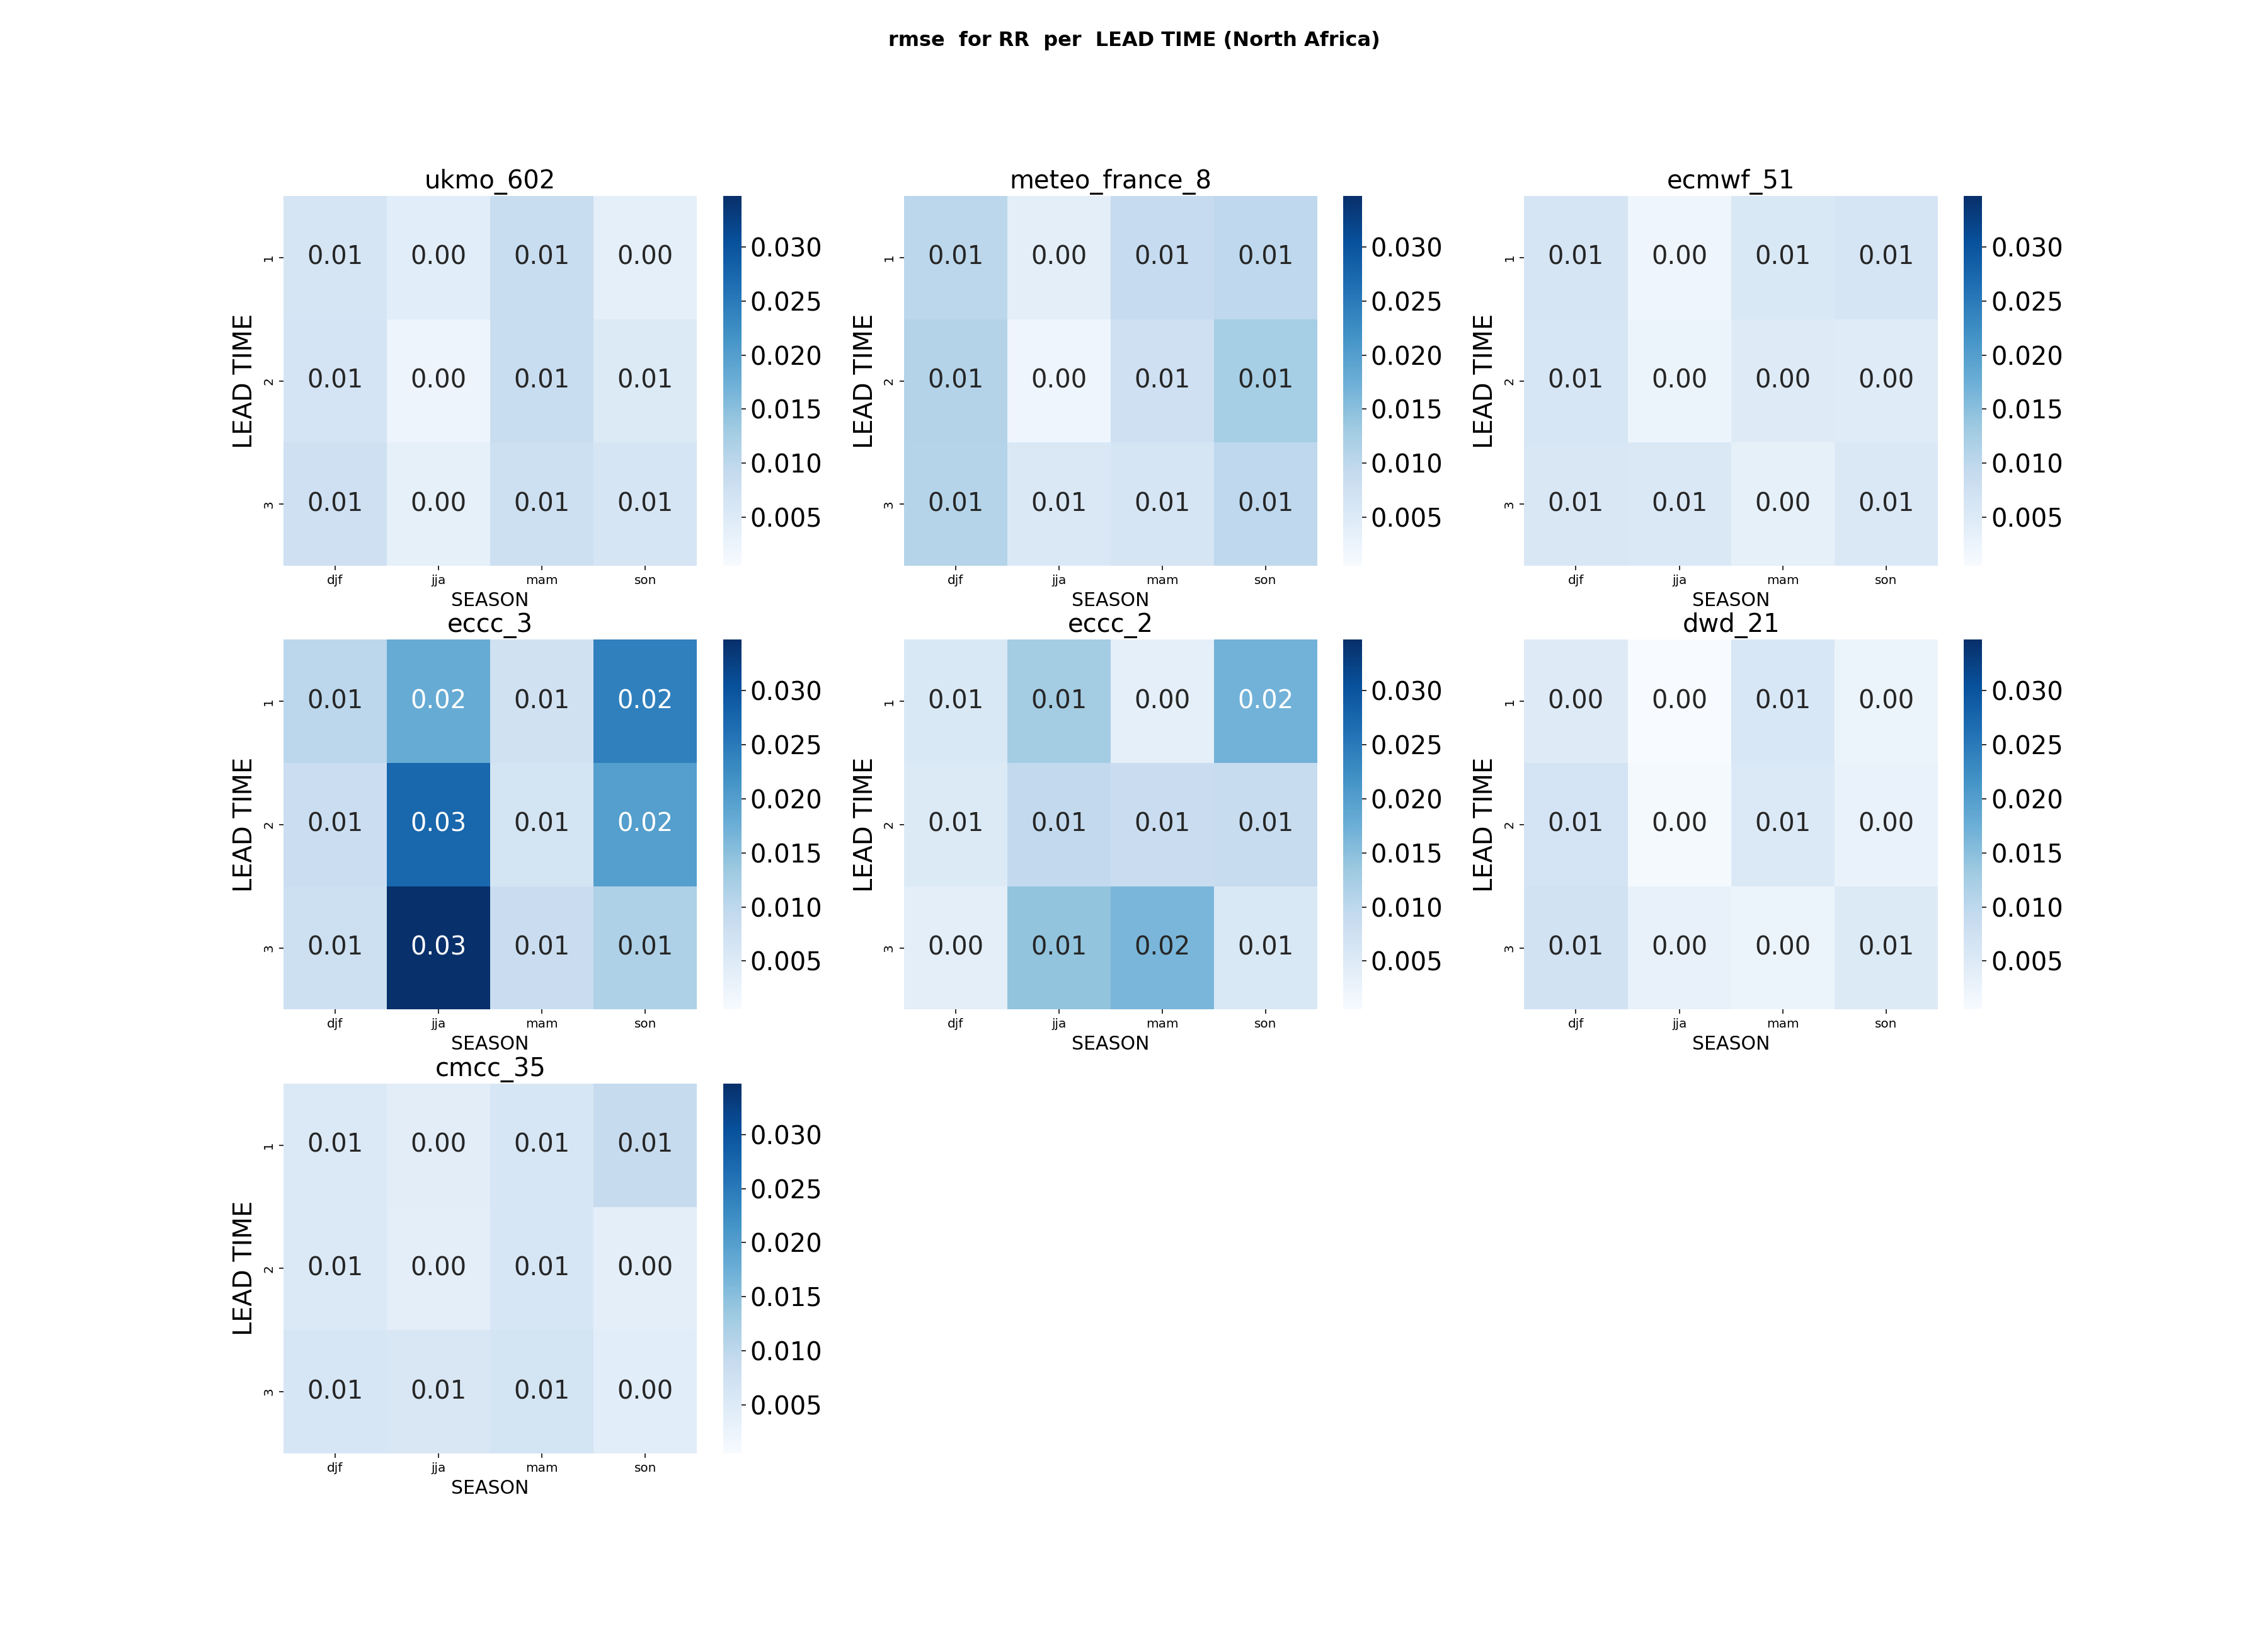
\includegraphics[scale=0.3]{plots/det/rmse/rmse_RR_NorthAfrica.png}
\caption{heatmap of RMSE For RR in mm (North Africa)}
\end{figure}

the RMSE is much better for North africa, the score is good over all lead-times and seasons. The centers, \textbf{\textit{ecmwf, ukmo and dwd}} show very good performance.

\vspace{1.5cm}
\paragraph{focus on Arabian Peninsula}:

\begin{figure}[H]
\centering
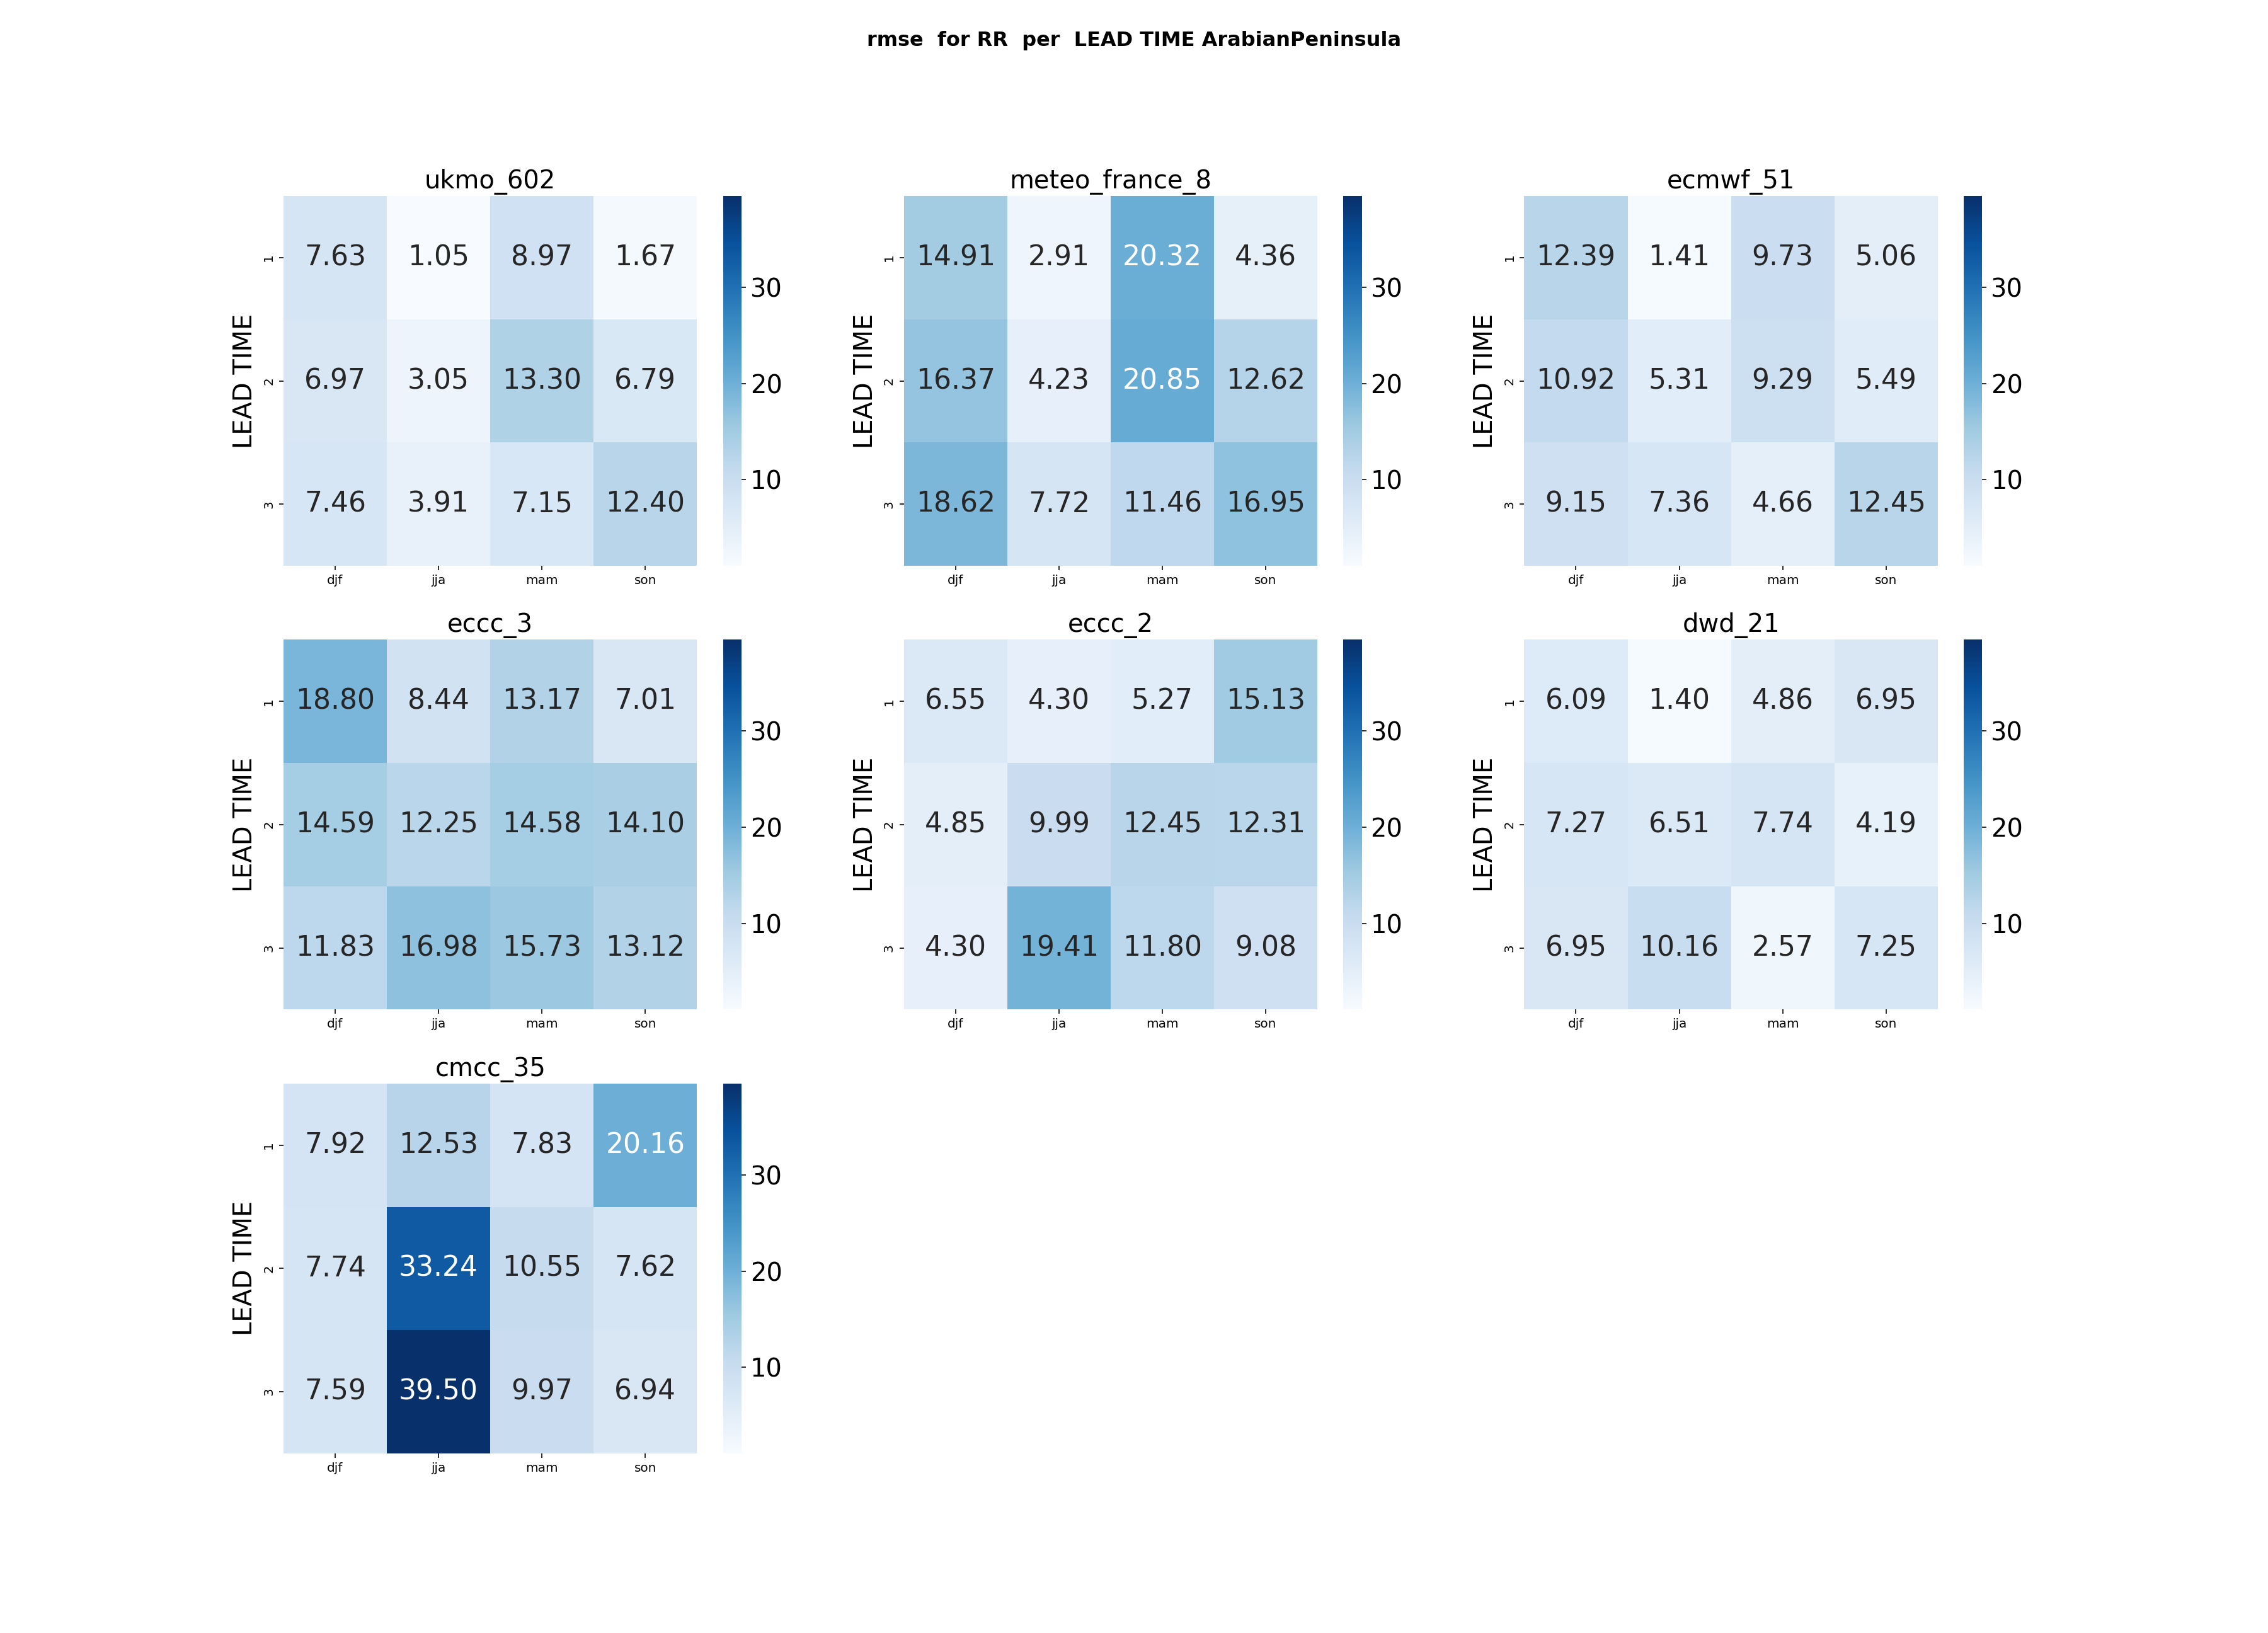
\includegraphics[scale=0.3]{plots/det/rmse/rmse_RR_ArabianPeninsula.png}
\caption{heatmap of RMSE For RR in mm (Arabian Peninsula)}
\end{figure}

In the same way as North Africa, the RMSE for the Arabian Peninsula is much better than mena. The centers, \textbf{\textit{ecmwf, ukmo and dwd}} show very good performance.

\subsubsection{Analysis of Coefficient of Determination results}

\paragraph{focus on North Africa}

there is no big difference in North Africa.


\vspace{1.5cm}
\paragraph{focus on Arabian Peninsula}:


\begin{figure}[H]
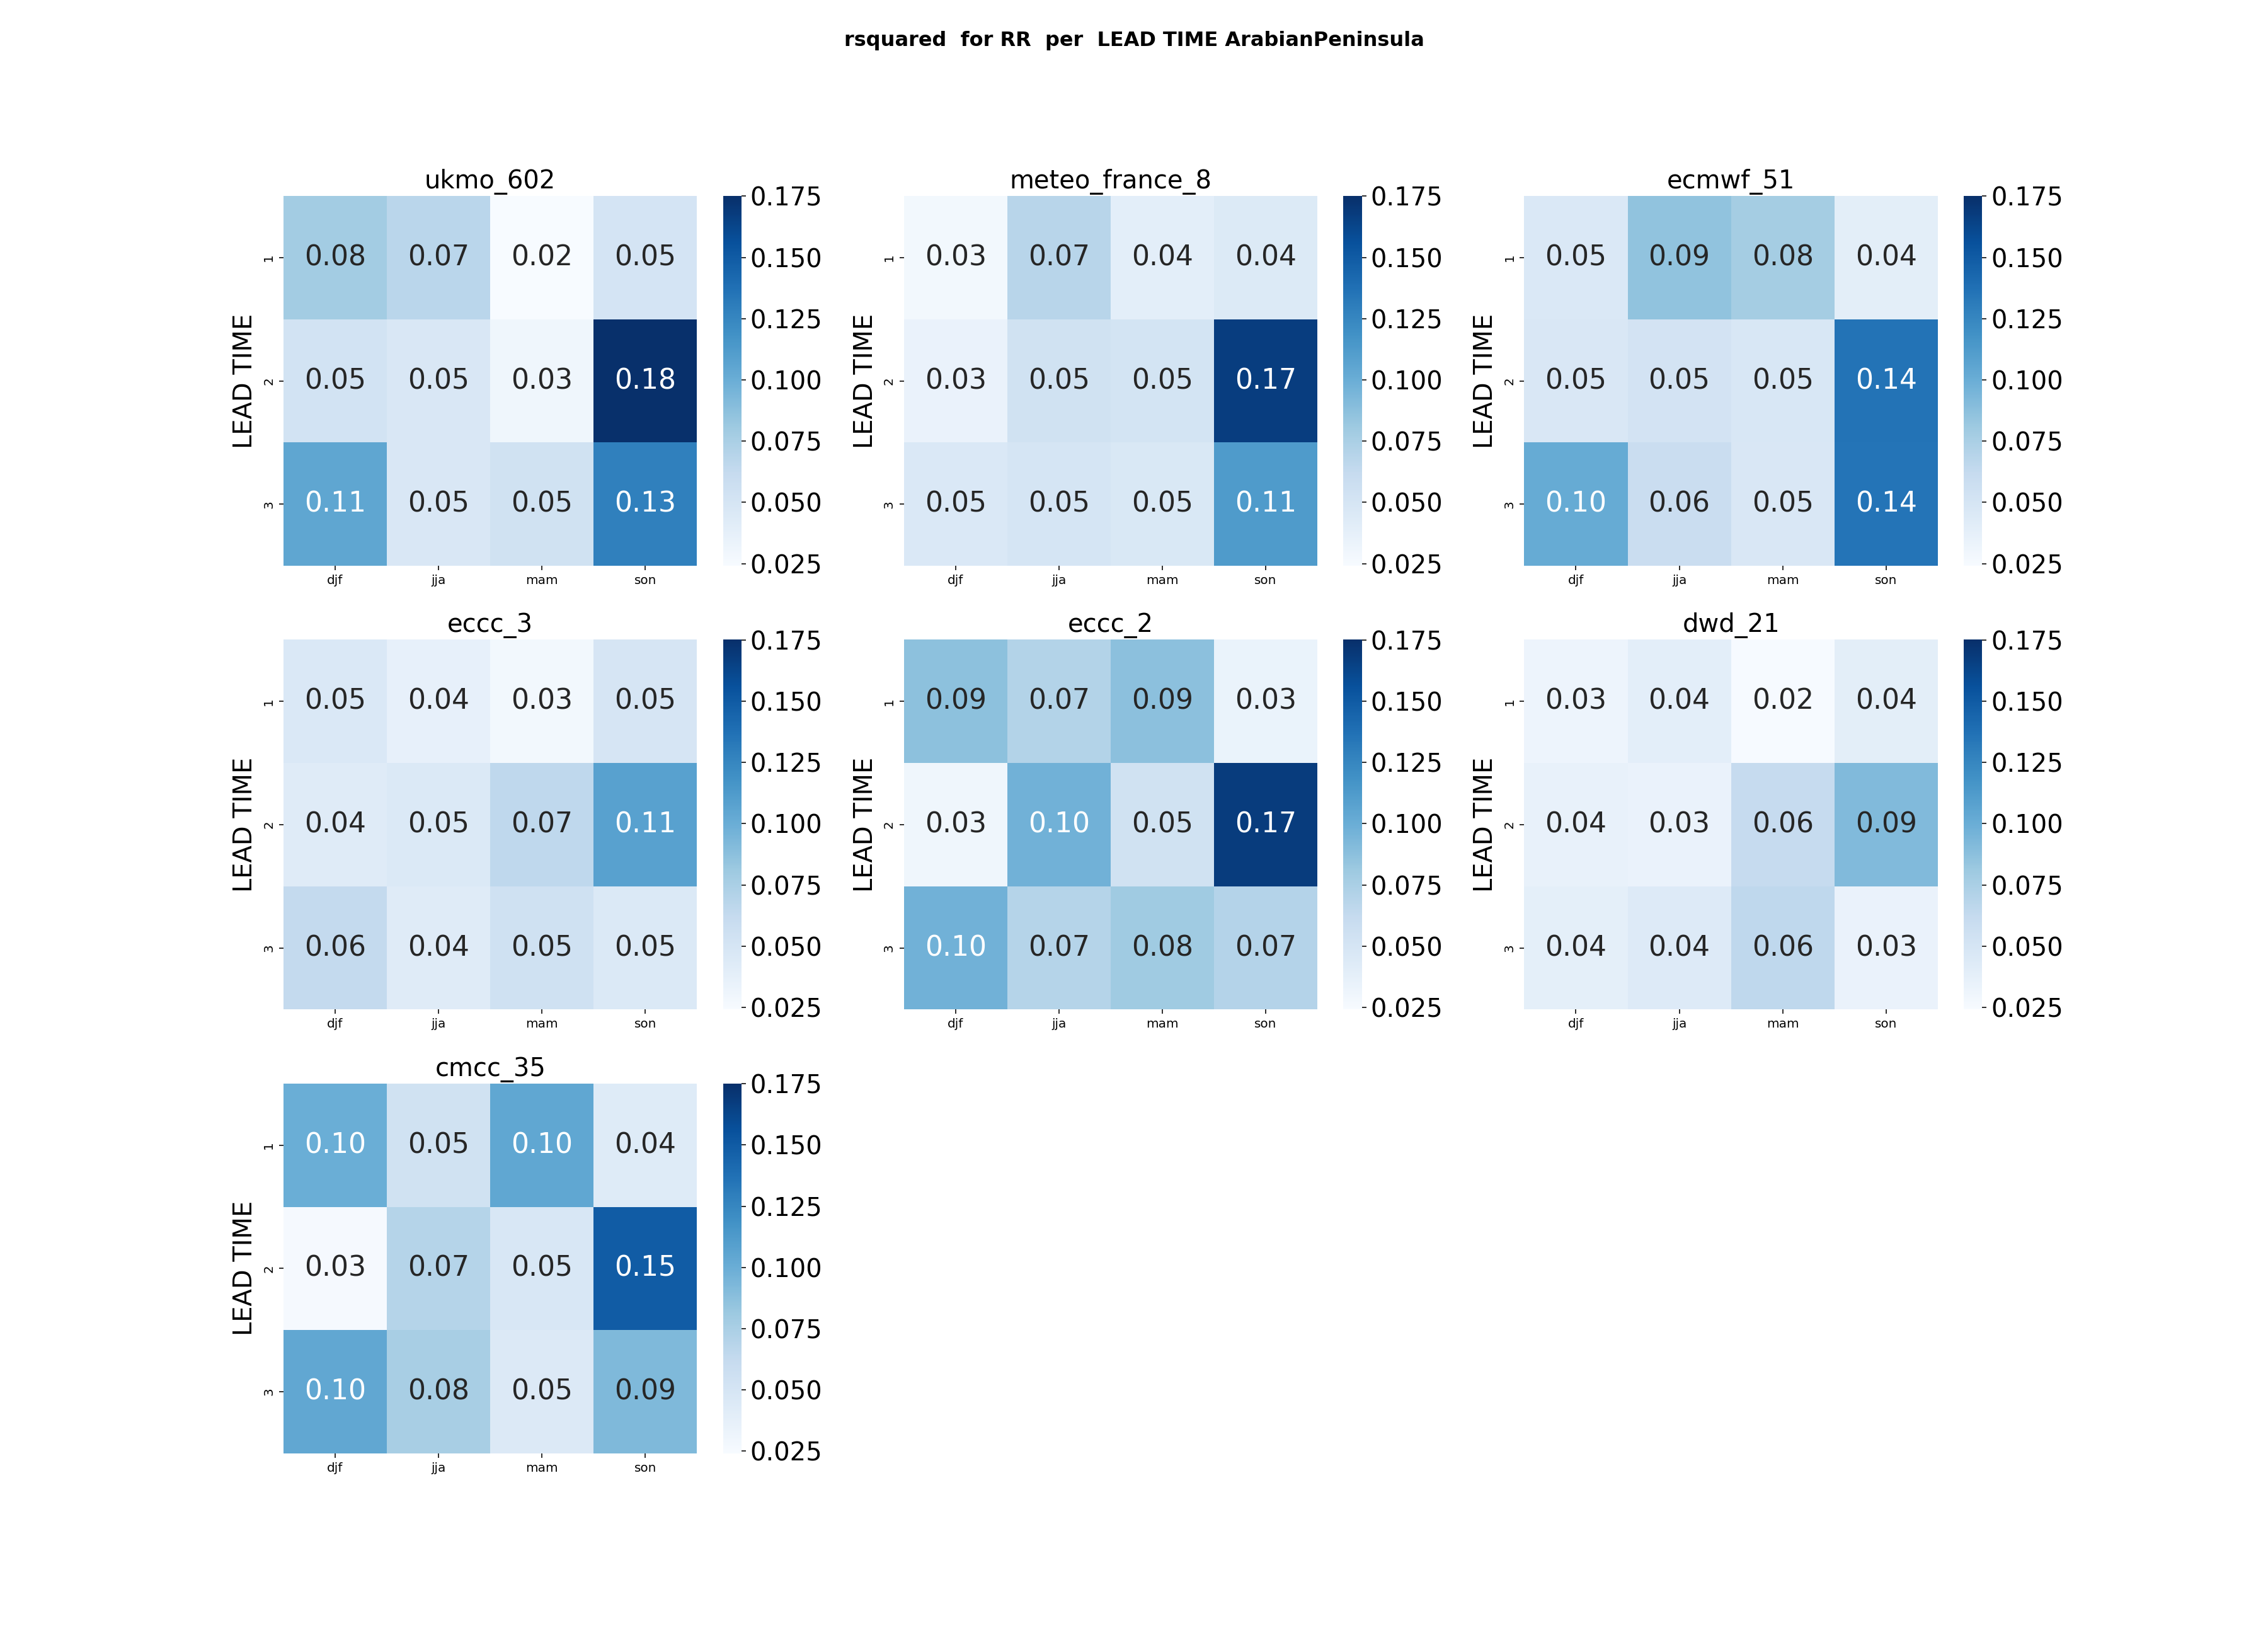
\includegraphics[scale=0.3]{plots/det/rsquared/rsquared_RR_ArabianPeninsula.png}
\caption{Heatmap of RR  RSQUARED in MENA Region for all centers Arabian Peninsula}
\end{figure}

the R-SQUARED for the Arabian Peninsula shows a little improvement.

\subsection{Probabilistic Evaluation Metrics}

\subsubsection{Analysis of The Brier Score results}

\paragraph{focus on North Africa}:

there is no big difference in North Africa.
\vspace{1.5cm}
\paragraph{focus on Arabian Peninsula}:
there is no big difference in North Africa.

\subsubsection{ Analysis of Reliability results}
\paragraph{focus on North Africa}:

there is no big difference in North Africa.

\paragraph{focus on Arabian Peninsula}:




\begin{figure}[H]
    \centering
    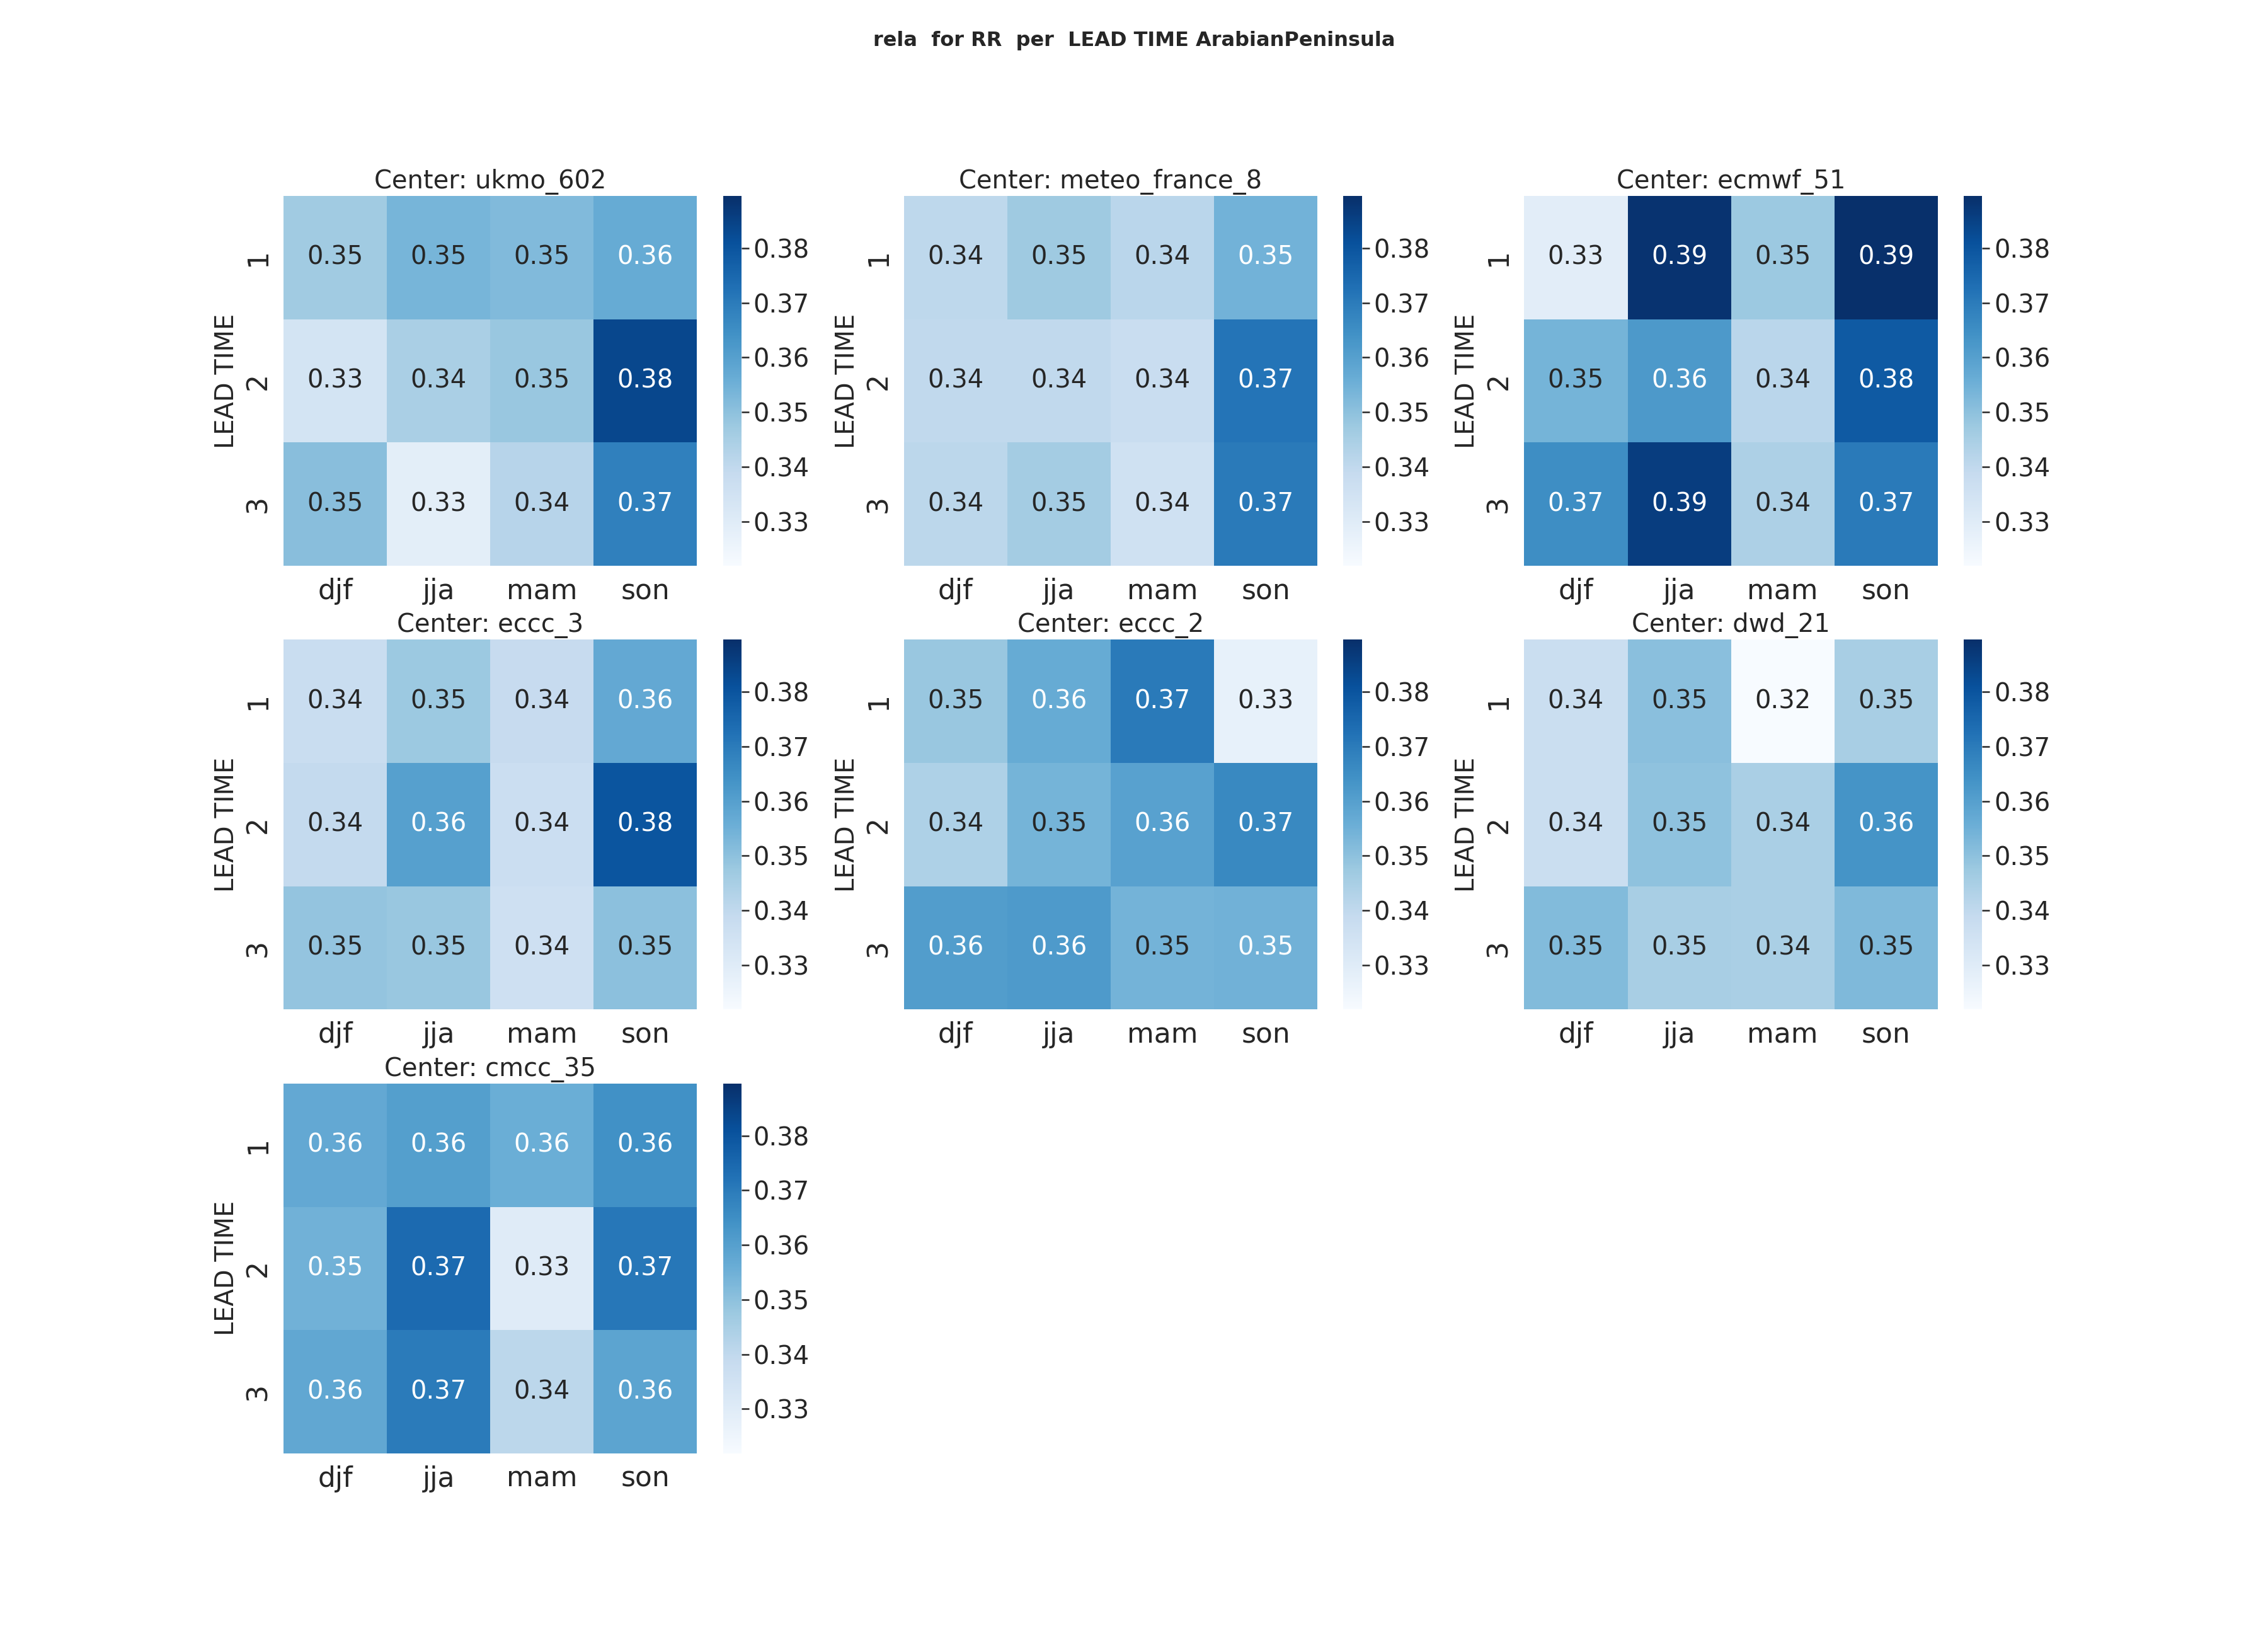
\includegraphics[scale=0.25]{plots/prob/rela/rela_RR_ArabianPeninsula.png}
    \caption{The Reliability Score Arabian Peninsula . \textbf{\textit{(0 means perfect Reliability )}}}
\end{figure}

There is a little Decline in the reliability of the Arabian Peninsula, especially f\textbf{\textit{ukmo}}

\subsubsection{Analysis of The ranked probability score results}
\paragraph{focus on north africa:}

there is no big difference in North Africa.

\paragraph{focus on Arabian Peninsula}:

there is no big difference on Arabian Peninsula.
\subsubsection{Analysis of Receiver Operating Characteristic results}
\paragraph{focus on north africa:}

there is no big difference in North Africa.
	
\paragraph{focus on Arabian Peninsula}:



\begin{figure}[H]
    \centering
    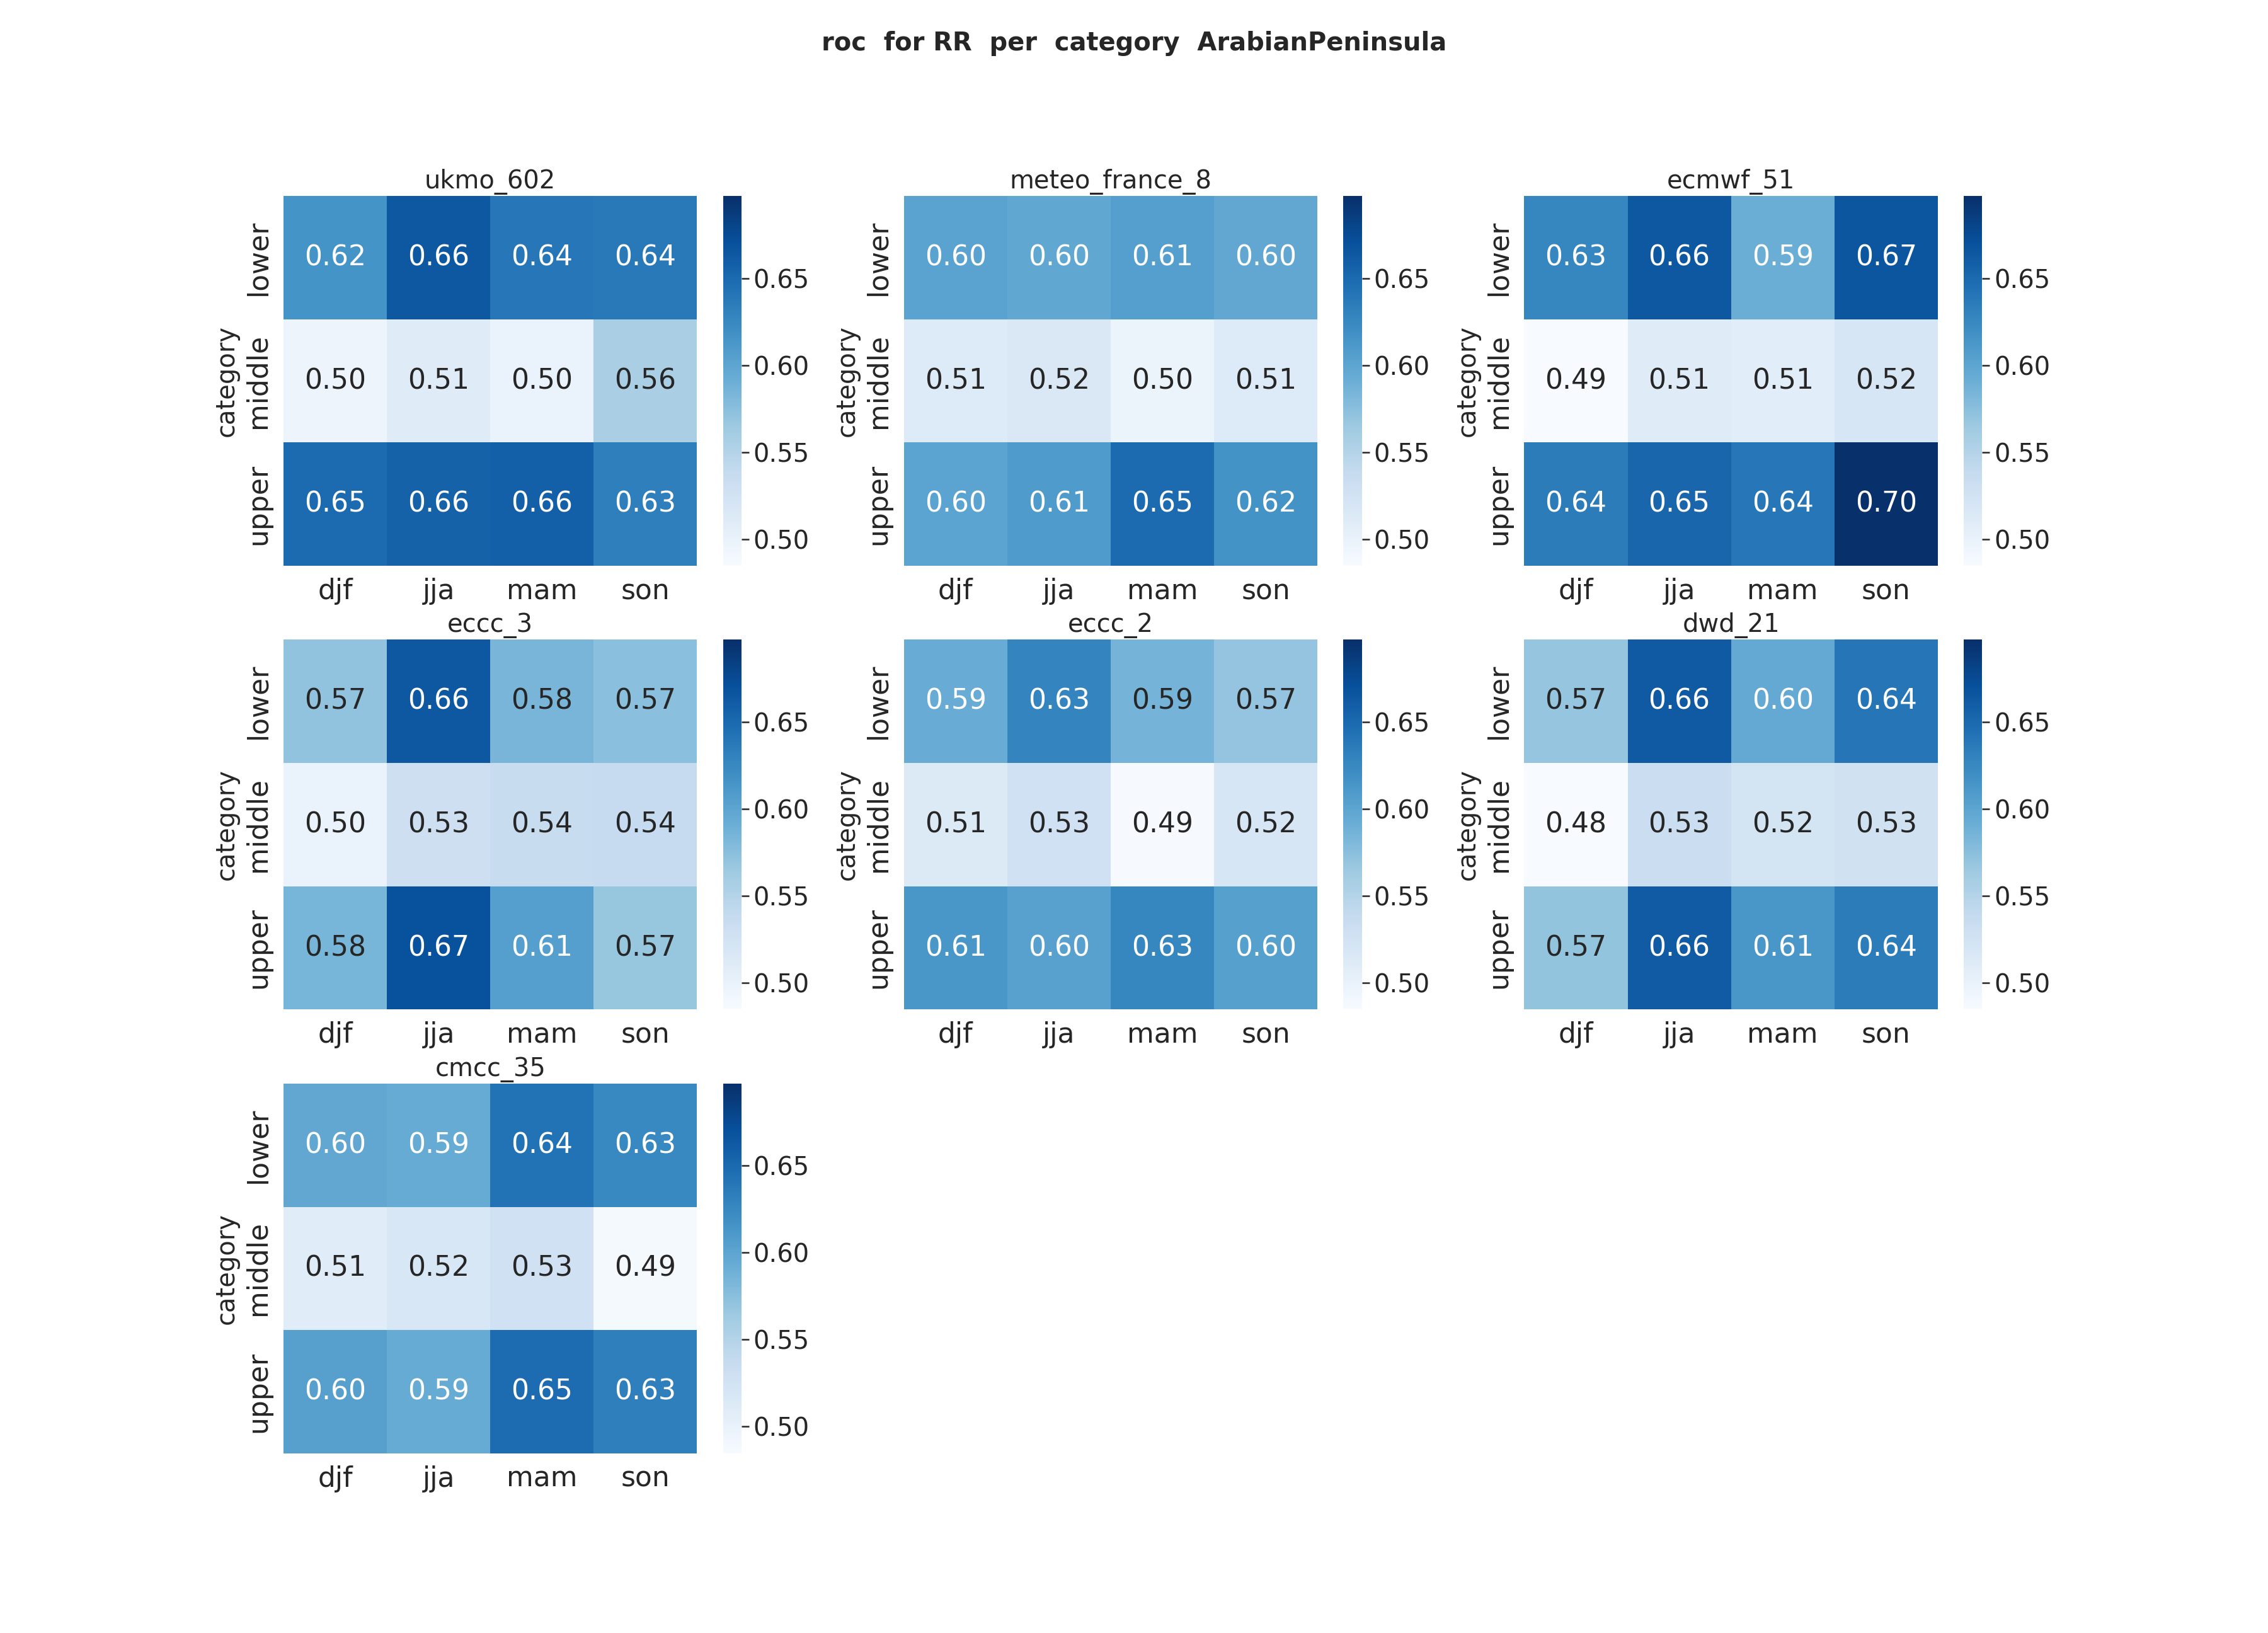
\includegraphics[scale=0.25]{plots/prob/roc/roc_RR_category_ArabianPeninsula.png}
    \caption{The ROC Score for each category Arabian Peninsula . \textbf{\textit{(1 means perfect ROC)}}}
\end{figure}


\begin{figure}[H]
    \centering
    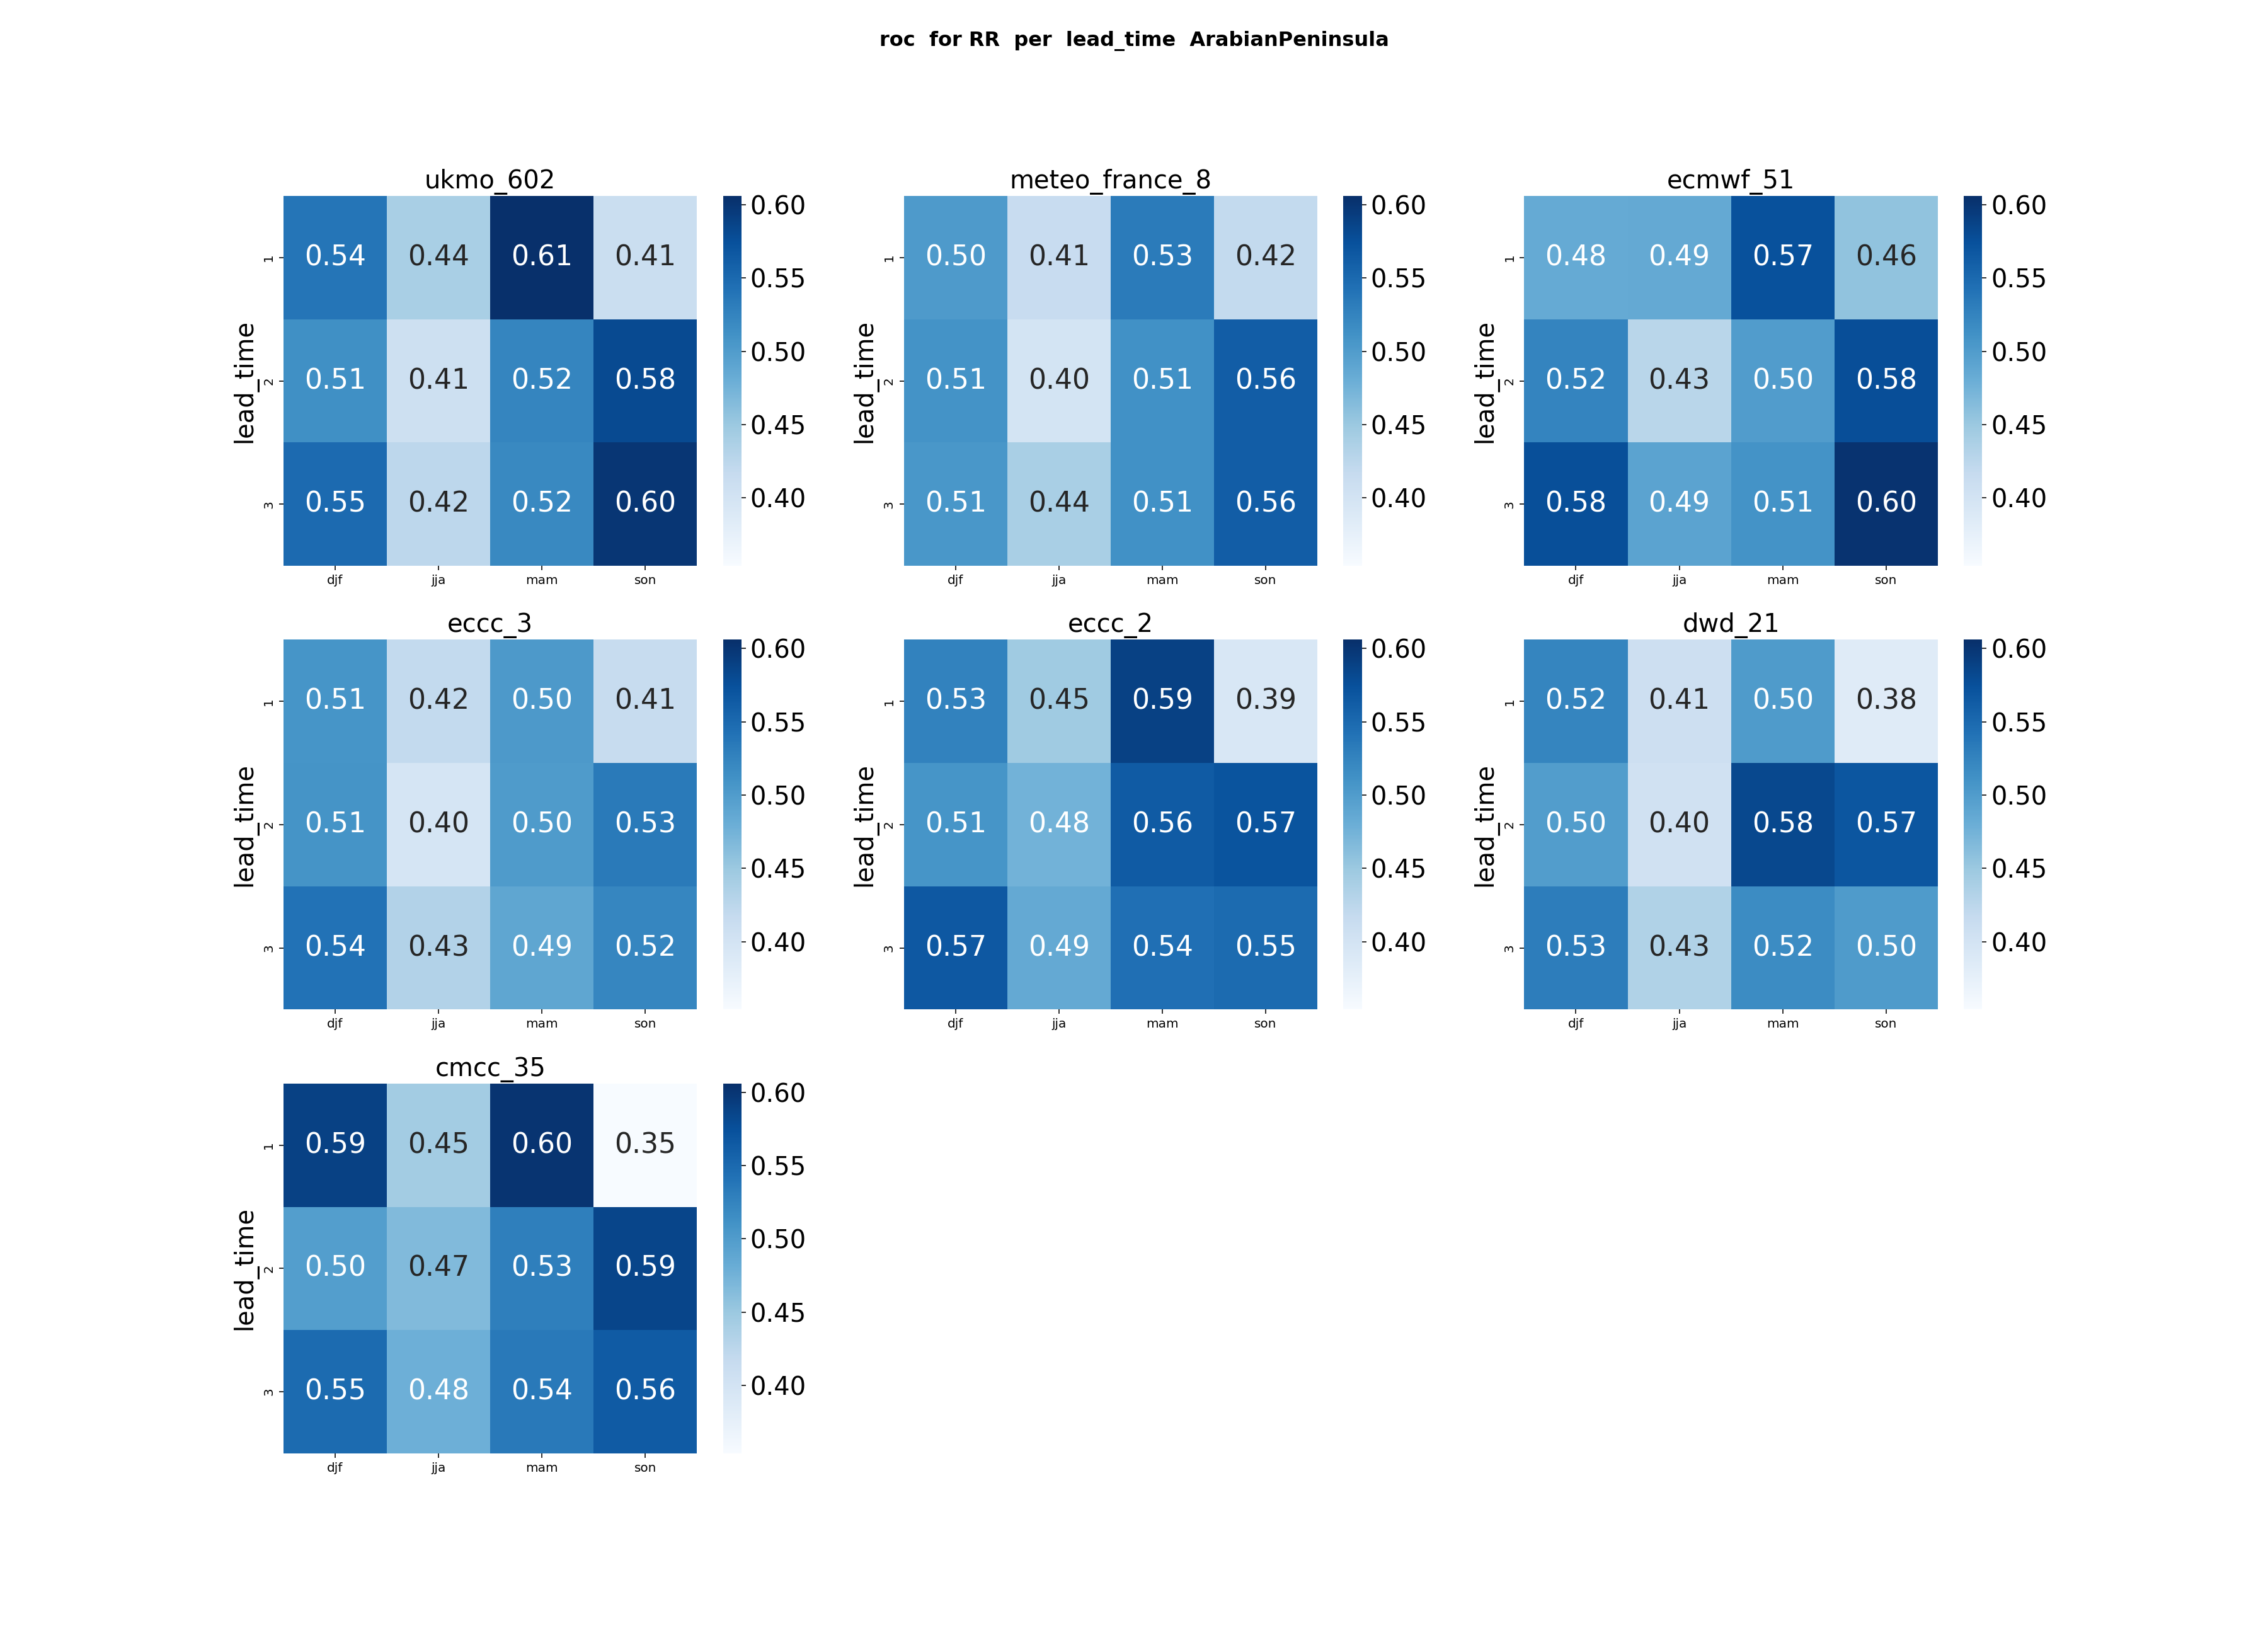
\includegraphics[scale=0.25]{plots/prob/roc/roc_RR_lead_time_ArabianPeninsula.png}
    \caption{The average of  ROC Score on all categories for Arabian Peninsula . \textbf{\textit{(1 means perfect ROC)}}}
\end{figure}


For the roc score, the focus on Arabian Peninsula in category, show no big difference, as for the analysis along lead-time, there is a few improvement for DJF, MAM and SON, instead of JJA that shows low values for all centers. 													\subsubsection{Analysis of Relative operating characteristics Skill Score results }
\paragraph{focus on north africa:}
\begin{figure}[H]
    \centering
    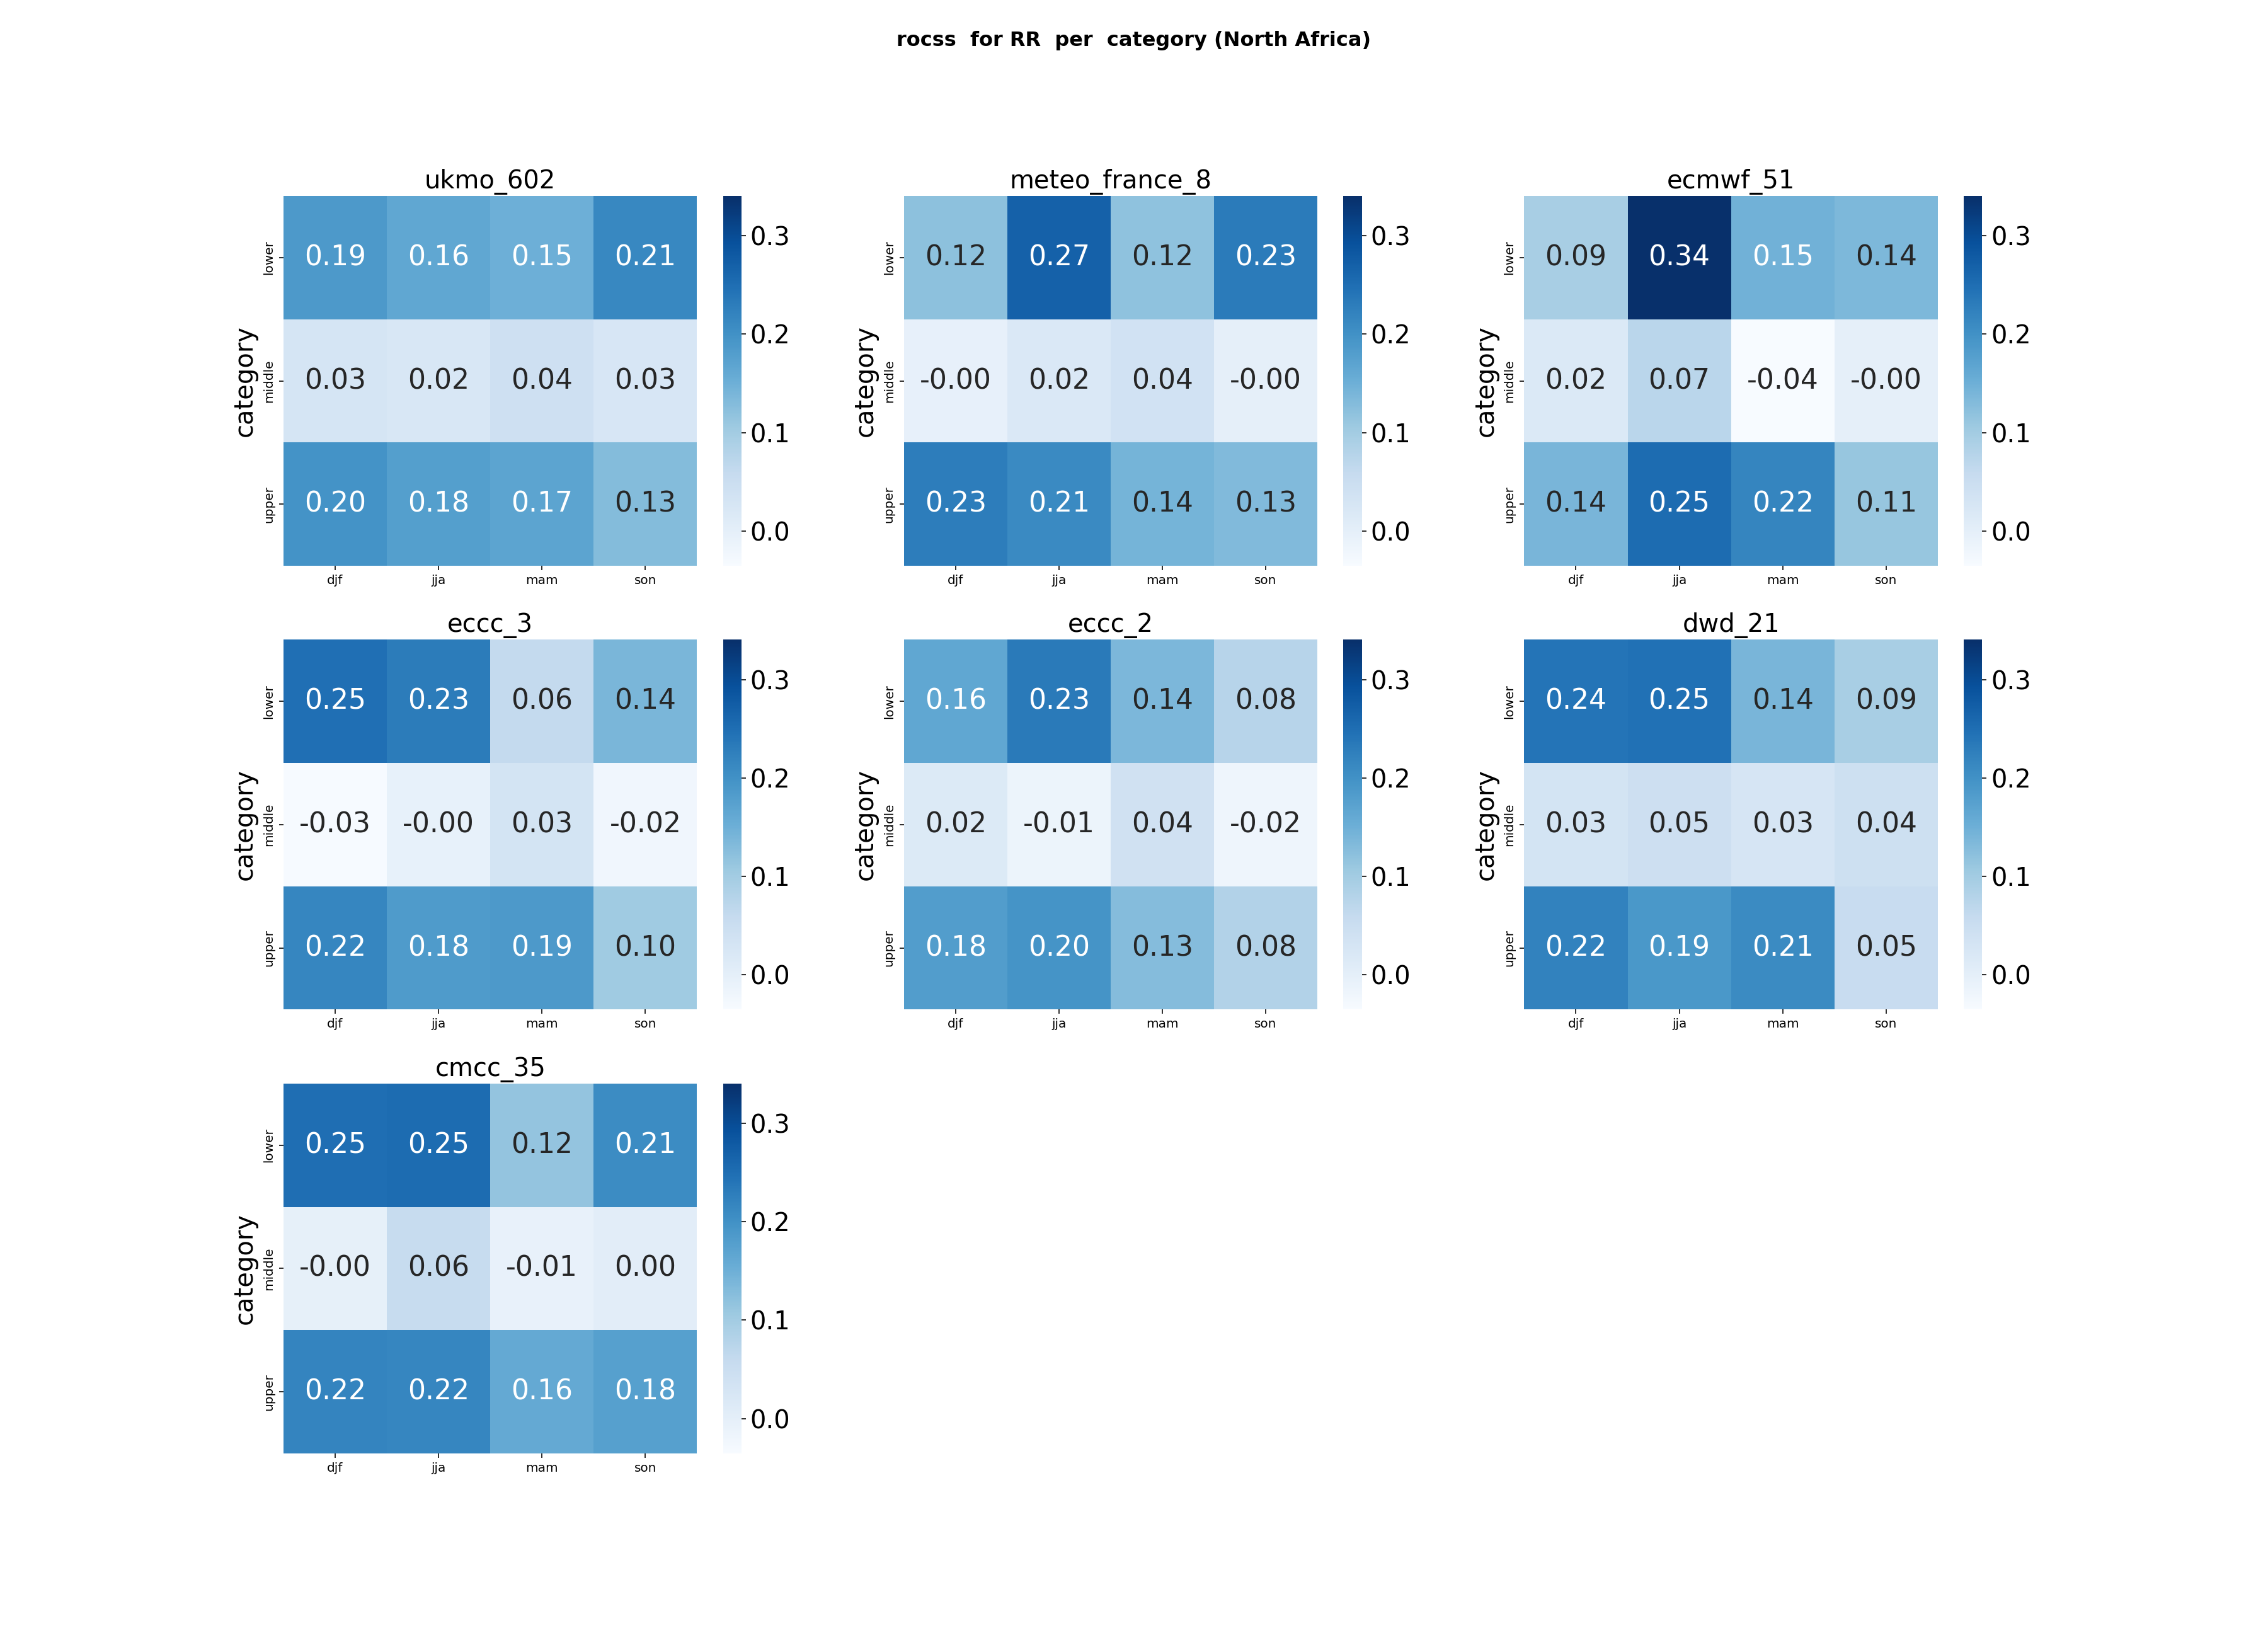
\includegraphics[scale=0.25]{plots/prob/rocss/rocss_RR_category_NorthAfrica.png}
    \caption{The ROCSS Score for each category North Africa . \textbf{\textit{(1 means perfect ROCSS)}}}
\end{figure}


\begin{figure}[H]
    \centering
    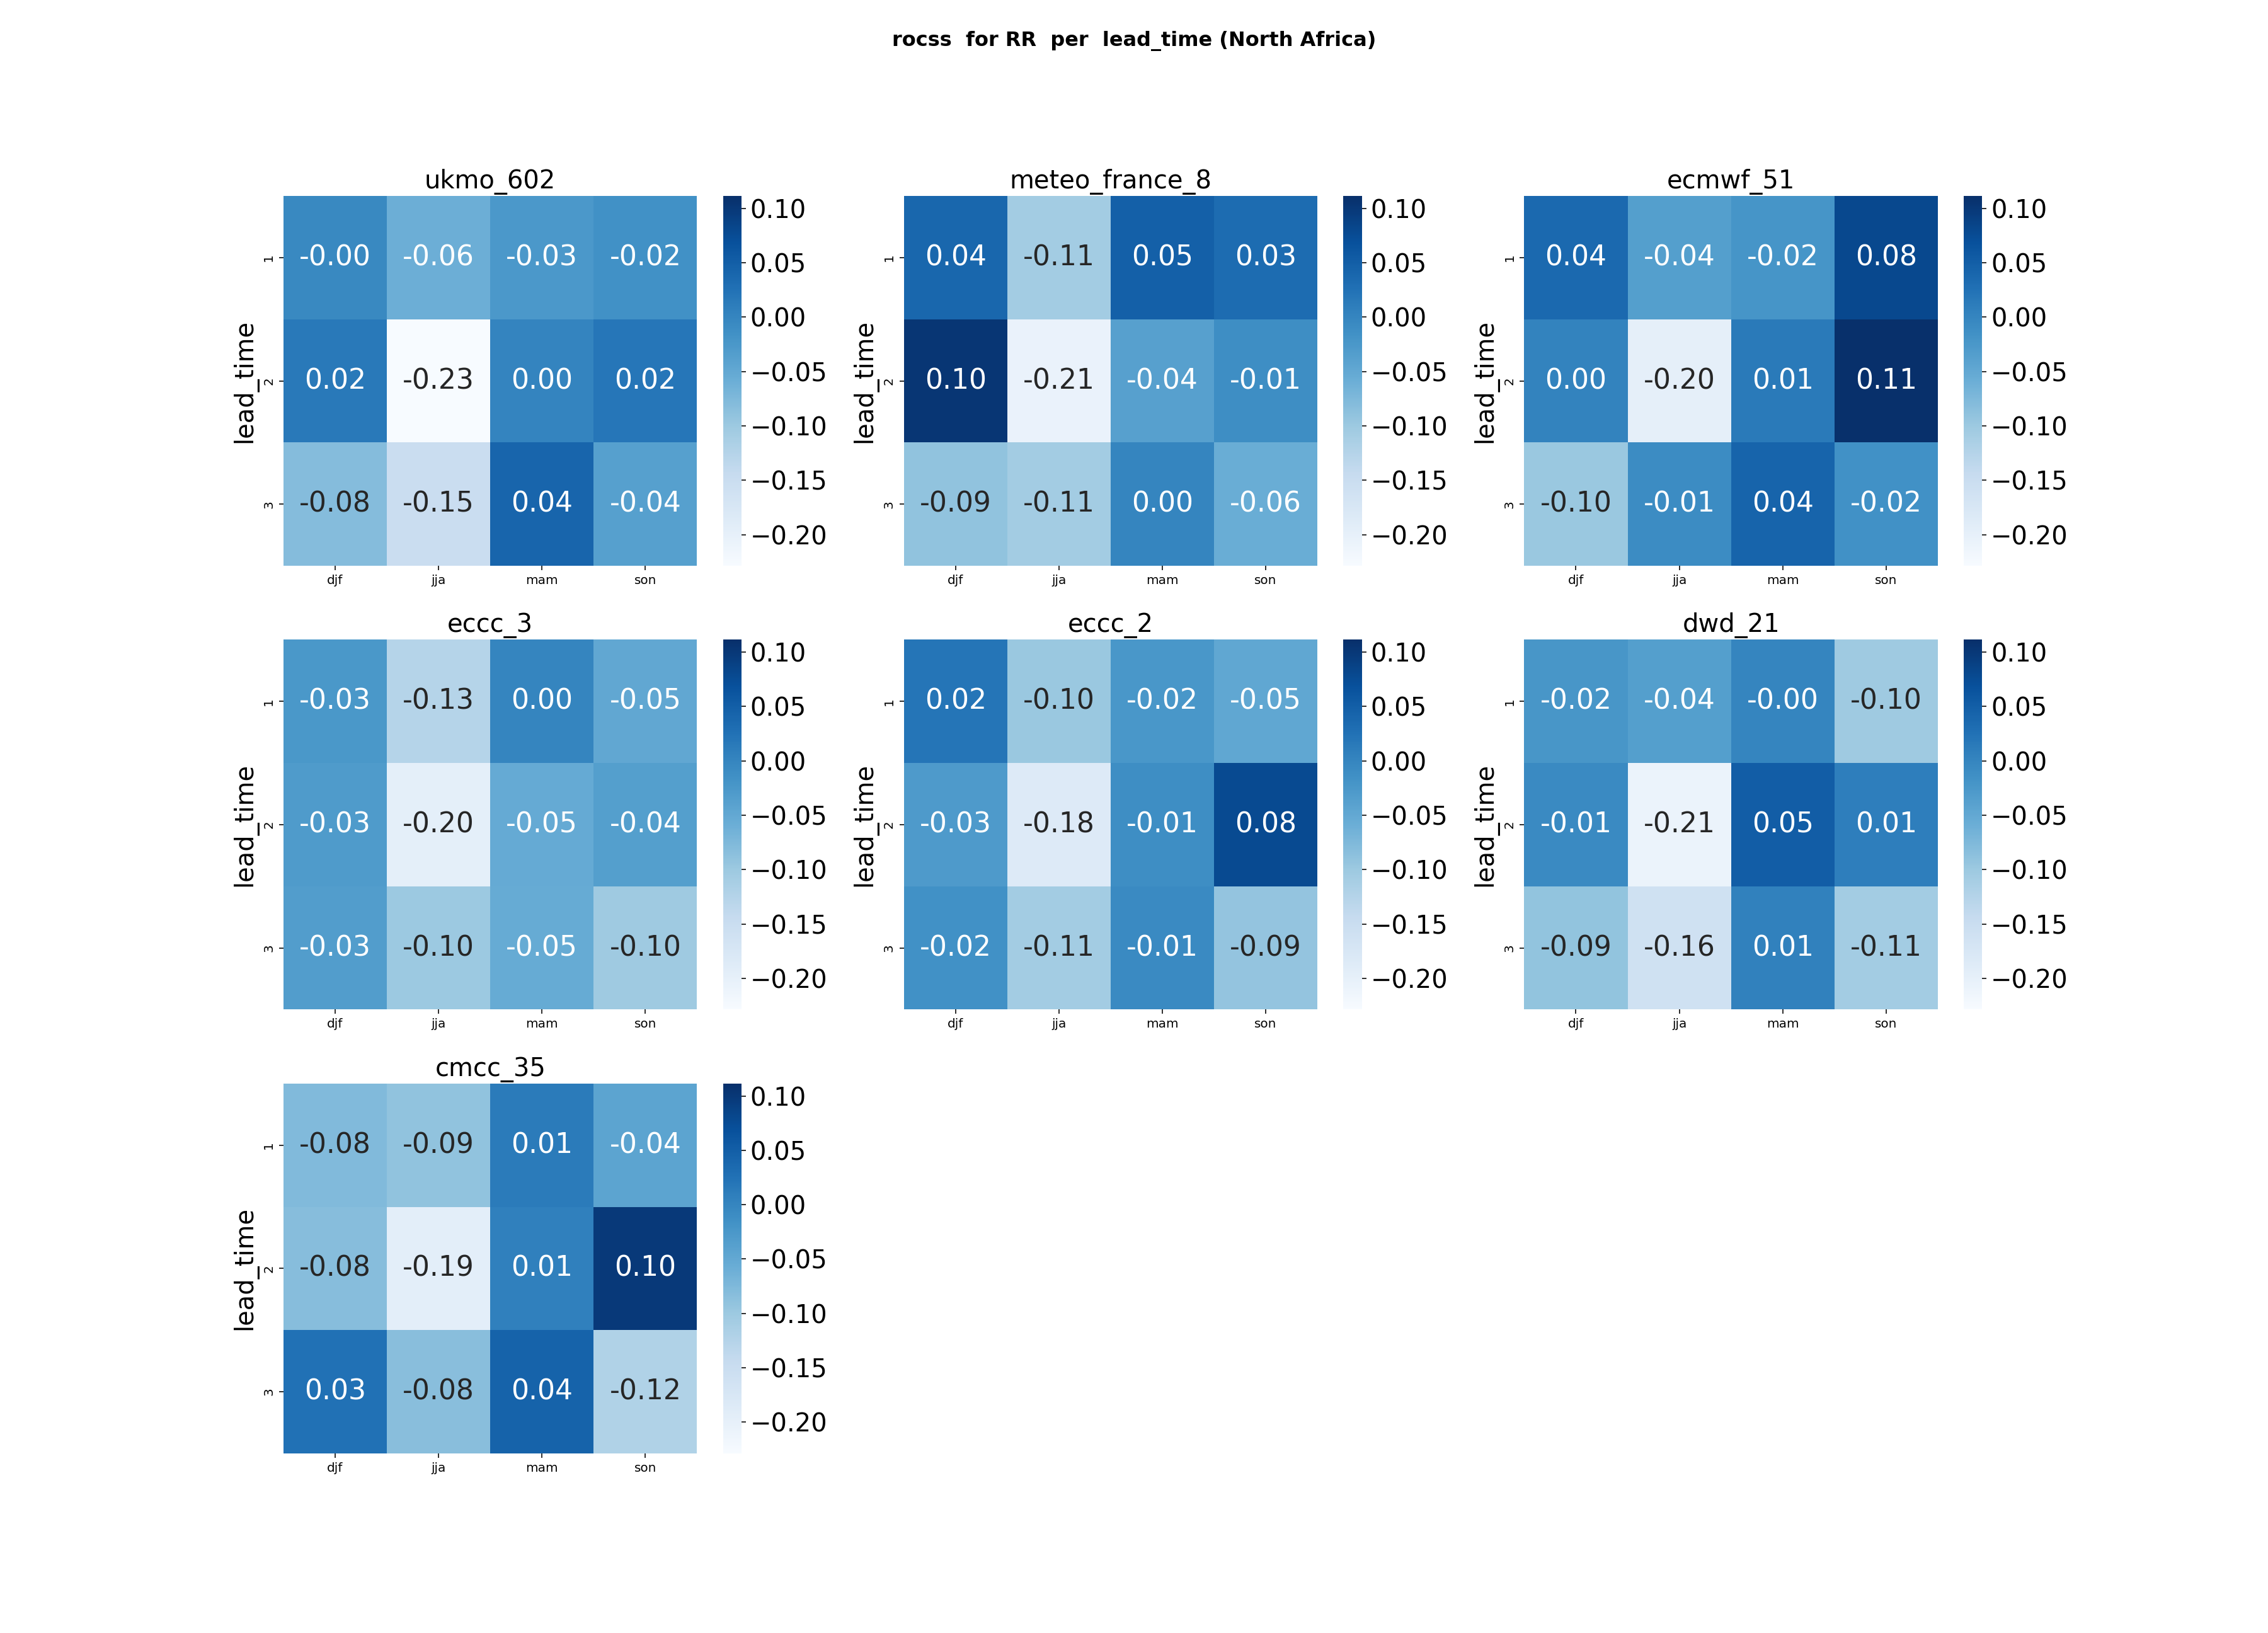
\includegraphics[scale=0.25]{plots/prob/rocss/rocss_RR_lead_time_NorthAfrica.png}
    \caption{The average of  ROCSS Score on all categories North Africa   . \textbf{\textit{(1 means perfect ROCSS)}}}
\end{figure}


the rocss for North Africa is in general lower, thus the performance is less accurate.

\paragraph{focus on Arabian Peninsula}:
\begin{figure}[H]
    \centering
    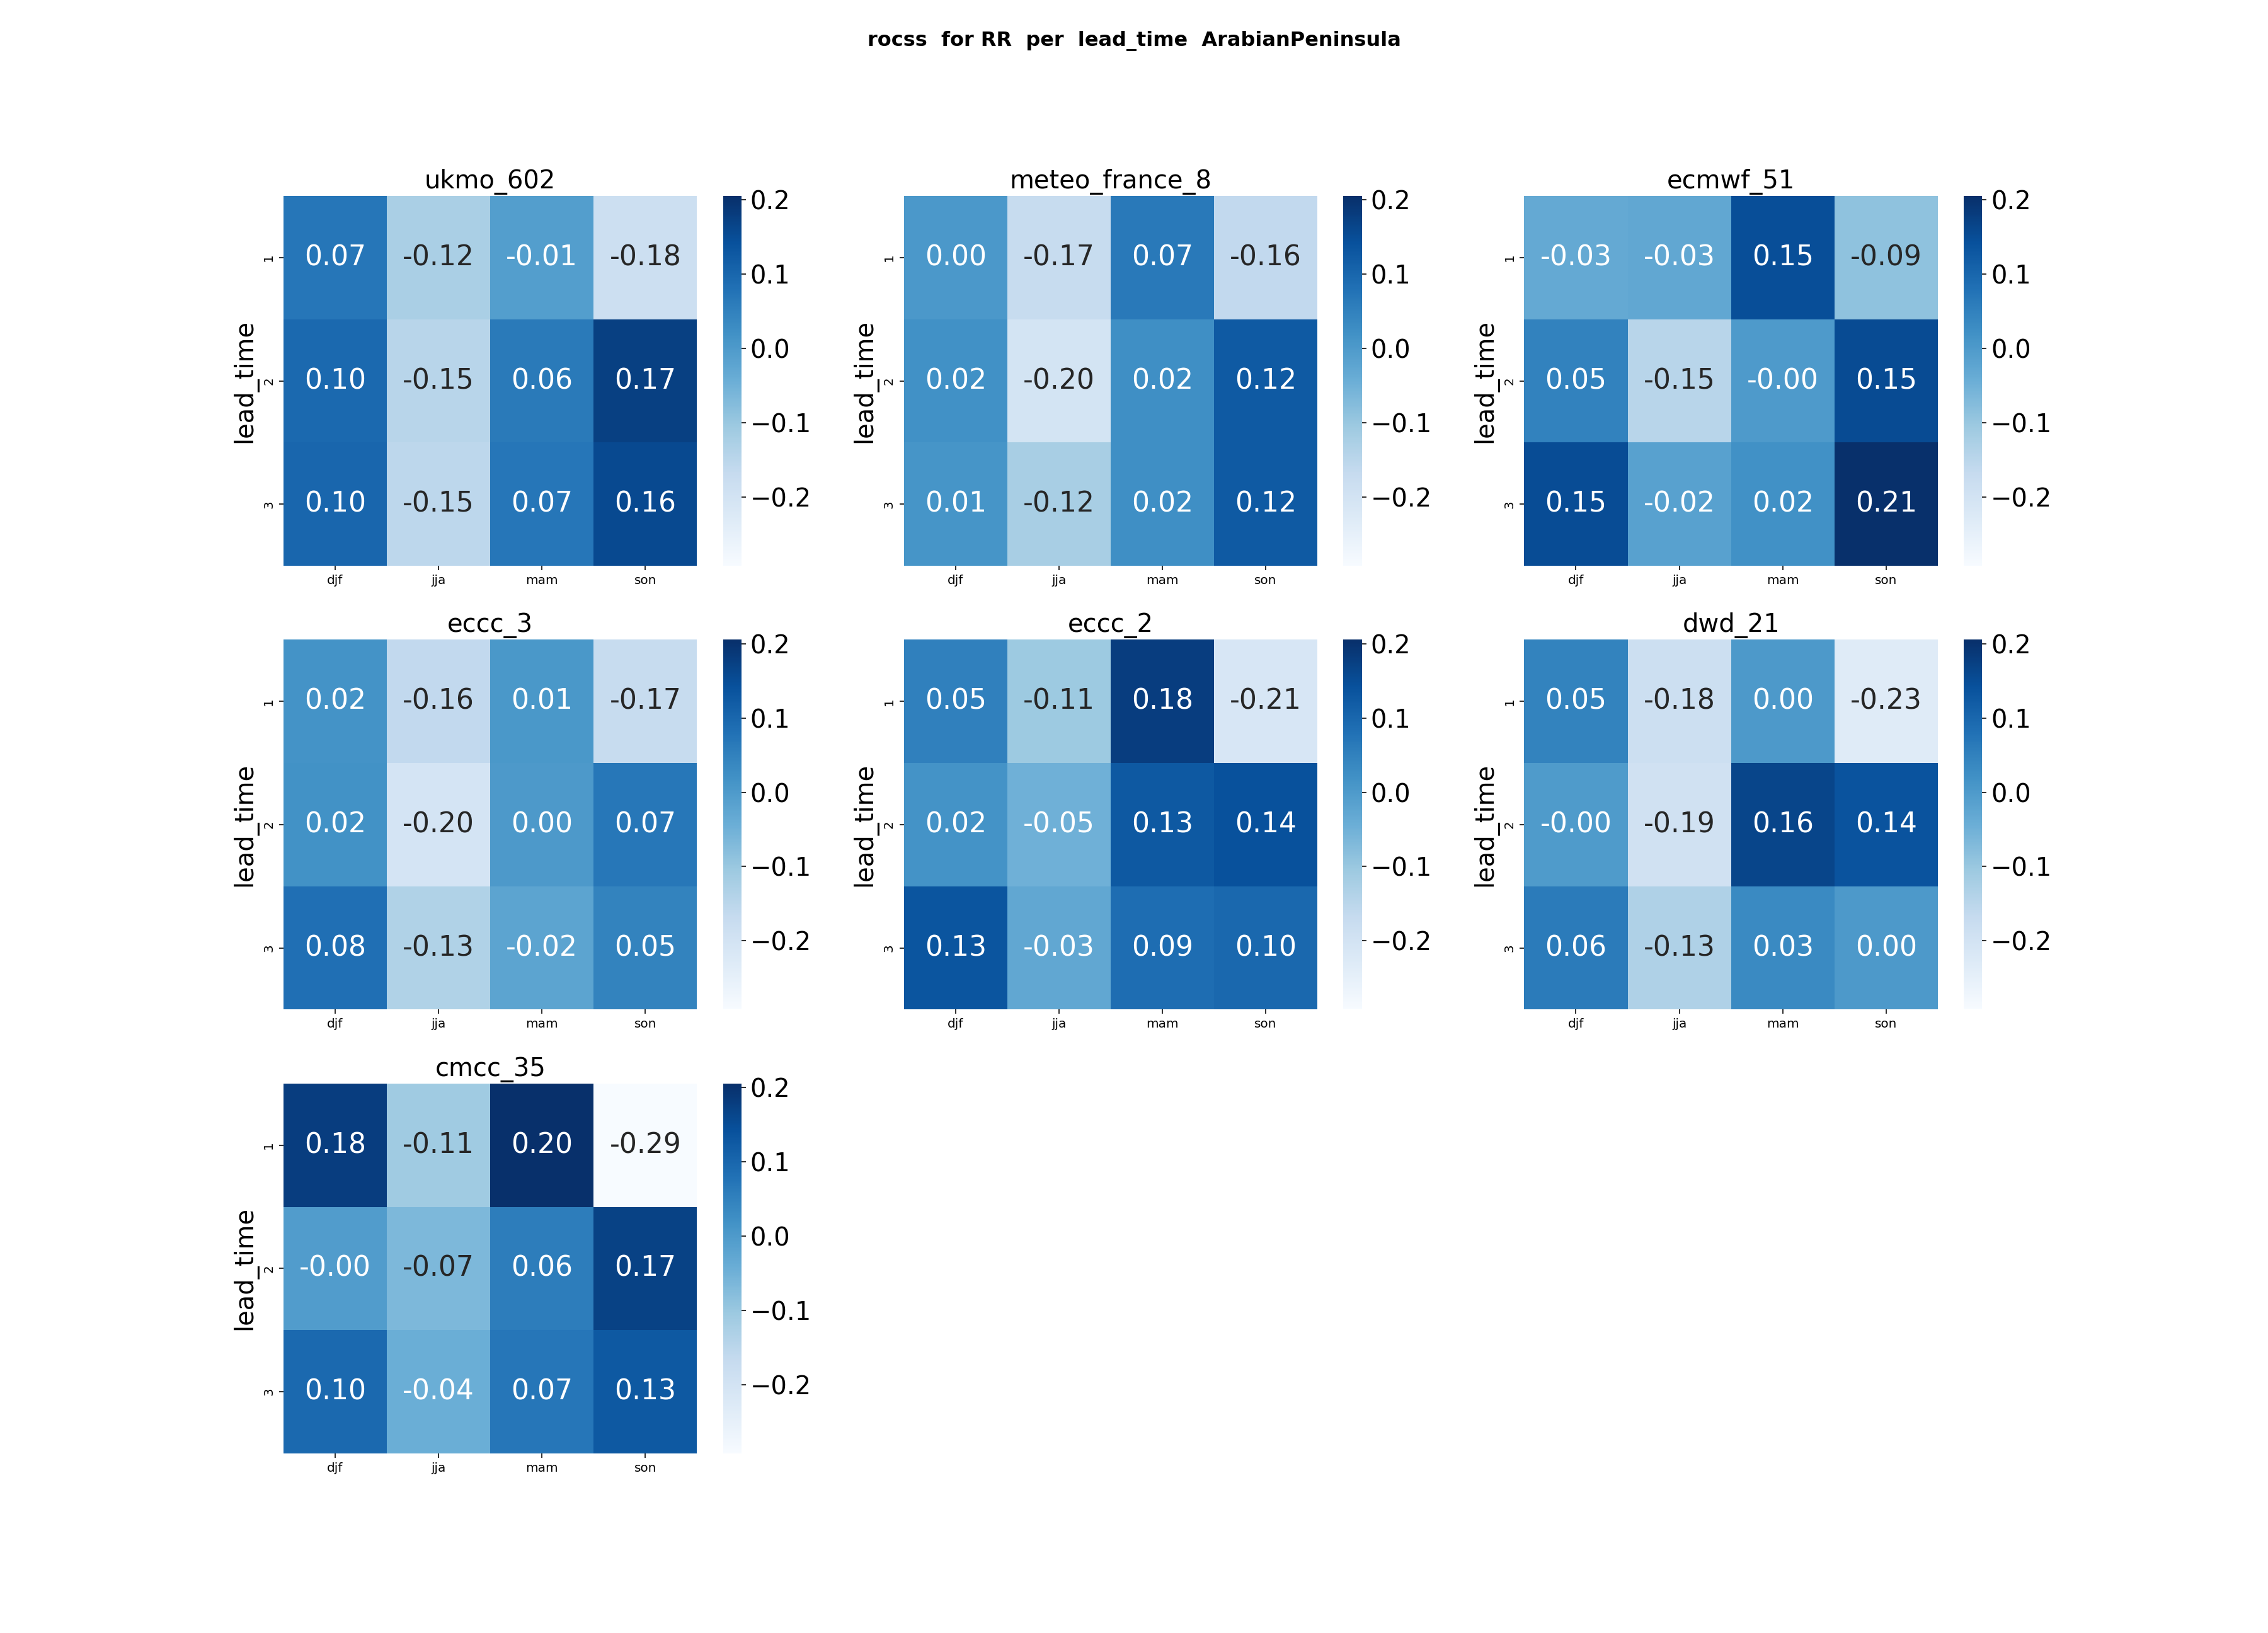
\includegraphics[scale=0.25]{plots/prob/rocss/rocss_RR_lead_time_ArabianPeninsula.png}
    \caption{The average of  ROCSS Score on all categories for Arabian Peninsula . \textbf{\textit{(1 means perfect ROCSS)}}}
\end{figure}


the rocss for Arabian Peninsula is in general lower, thus the performance is less accurate.


